\documentclass[aspectratio=169]{beamer}
\IfFileExists{beamerthememetropolis.sty}{\usetheme{metropolis}}{\usetheme{default}}
\usepackage[utf8]{inputenc}
\usepackage[T1]{fontenc}
\usepackage{booktabs}
\usepackage{graphicx}
\usepackage{amsmath}
\usepackage{xcolor}
\usepackage{tikz}
\definecolor{shipblue}{RGB}{20,74,130}
\definecolor{warningorange}{RGB}{210,105,30}
\setbeamercolor{structure}{fg=shipblue}
\setbeamercolor{alerted text}{fg=warningorange}
\setbeamertemplate{navigation symbols}{}
\title{EXEC\_09: EndTop photon budget and intrinsic timing}
\subtitle{Tail-drain mechanism, validated 86-channel coverage study}
\author{Rene Rios (ULS)}
\date{June 10, 2026}
\begin{document}
\begin{frame}{Configuration and provenance}

\begin{columns}[T]\column{0.62\textwidth}
\textbf{Branch:} \texttt{feat/endtop-sslg4}\\
\textbf{Commits:} \texttt{1f6aca1}, \texttt{9613fc9}, final EXEC\_09 deliverable commit
\begin{itemize}\small
  \item 31 positions $\times$ 2000 events; 16 End + 70 Top channels; jitter fixed to zero.
  \item EJ-204 via SSLG4 \texttt{OPSC-101}: yield 10400/MeV, $\tau_r=0.7$ ns,
        $\tau_d=1.8$ ns, ABSLENGTH=160 cm (verified effective MPT inputs).
  \item Broadcom AFBR-S4N66P024M: PDE 63\% at 420 nm.
\end{itemize}
\column{0.35\textwidth}
\begin{alertblock}{Scope}
Top 70 SiPM is a simulation coverage study. Real hardware: 32 Top SiPMs.
All reported timing is intrinsic, without SPTR or electronics jitter.
\end{alertblock}
\end{columns}

\end{frame}
\begin{frame}{EndTop geometry and channel map}

\begin{columns}[T]\column{0.55\textwidth}
\begin{itemize}
 \item EJ-204 bar: $1400\times60\times10$ mm$^3$.
 \item End L IDs 0--7; End R IDs 8--15.
 \item Top L IDs 16--50: $-692,-672,\ldots,-12$ mm.
 \item Top R IDs 51--85: $+12,+32,\ldots,+692$ mm.
 \item Each Top element and window: $6\times6$ mm$^2$.
\end{itemize}
\column{0.42\textwidth}
\begin{block}{Exact constraints}
First centers are 5 mm from each bar end. Pitch is 20 mm except the deliberate
central $-12/+12$ mm pair, whose pitch is 24 mm.
\end{block}
\end{columns}

\end{frame}
\begin{frame}{Instrumented and wrapped faces}

\centering\begin{tabular}{lll}\toprule
Face & Optical state & Readout \\ \midrule
$-X$, $+X$ & open & 8 End SiPMs each \\
$+Y$ & Mylar with 70 exact windows & 70 Top SiPMs \\
$-Y$, $-Z$, $+Z$ & complete Mylar & none \\
\bottomrule\end{tabular}
\vspace{0.5cm}
\begin{block}{External layer}
Black Tedlar is deliberately not modeled; it only blocks ambient light.
The non-reflected Mylar fraction is already absorbed in the optical model.
\end{block}

\end{frame}
\begin{frame}{Window optics: why timing and collection change}

\centering
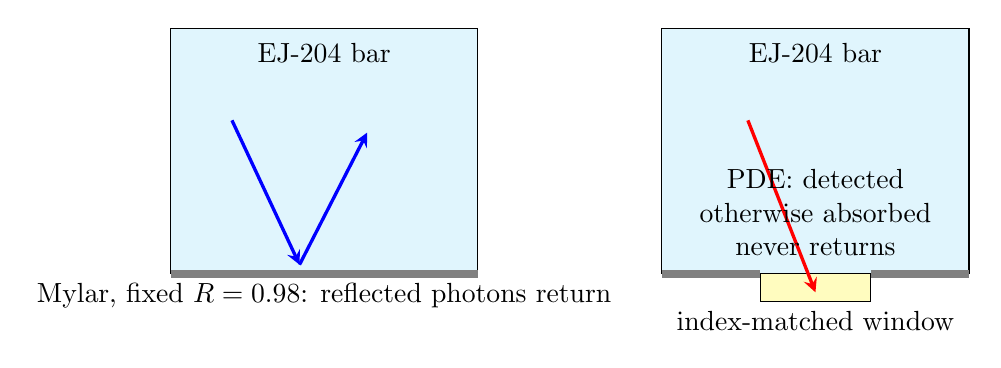
\begin{tikzpicture}[scale=0.78,>=stealth]
 \draw[fill=cyan!12] (0,0) rectangle (5,4);
 \node at (2.5,3.6) {EJ-204 bar};
 \draw[line width=3pt,gray] (0,0) -- (5,0);
 \node[below] at (2.5,0) {Mylar, fixed $R=0.98$: reflected photons return};
 \draw[->,very thick,blue] (1.0,2.5) -- (2.1,0.15);
 \draw[->,very thick,blue] (2.1,0.15) -- (3.2,2.3);
 \draw[fill=cyan!12] (8,0) rectangle (13,4);
 \node at (10.5,3.6) {EJ-204 bar};
 \draw[line width=3pt,gray] (8,0) -- (9.6,0);
 \draw[line width=3pt,gray] (11.4,0) -- (13,0);
 \draw[fill=yellow!25] (9.6,-0.45) rectangle (11.4,0);
 \node[below] at (10.5,-0.45) {index-matched window};
 \draw[->,very thick,red] (9.4,2.5) -- (10.5,-0.3);
 \node[align=center] at (10.5,1.0) {PDE: detected\\otherwise absorbed\\never returns};
\end{tikzpicture}
\begin{alertblock}{Consequence}
Every window is an optical drain. Long, multiply reflected paths have more chances
to meet one, so late End photons are preferentially removed.
\end{alertblock}

\end{frame}
\section{Position-by-position}
\begin{frame}{Position x=-690 mm}

\begin{columns}[T]
  \column{0.52\textwidth}
  
\includegraphics[width=\textwidth]{figs/muon_-690mm_geometry.png}
  \column{0.46\textwidth}
  
\includegraphics[width=\textwidth]{figs/muon_-690mm_top_profile.png}
  \scriptsize
  \begin{tabular}{lr}
    \toprule Quantity & Value \\ \midrule
    End L $N_{pe}$ & $3363.1\pm18.1$ \\
    End R $N_{pe}$ & $41.1\pm0.3$ \\
    Nearest Top ID & 16 (exact geometry) \\
    Nearest Top $N_{pe}$ & $350.9\pm2.0$ \\
    Nearest Top $\langle t\rangle$ &
      $2.786\pm0.002$ ns \\
    Nearest Top FPT & $0.343\pm0.000$ ns \\
    \bottomrule
  \end{tabular}
\end{columns}

\end{frame}
\begin{frame}{Position x=-670 mm}

\begin{columns}[T]
  \column{0.52\textwidth}
  
\includegraphics[width=\textwidth]{figs/muon_-670mm_geometry.png}
  \column{0.46\textwidth}
  
\includegraphics[width=\textwidth]{figs/muon_-670mm_top_profile.png}
  \scriptsize
  \begin{tabular}{lr}
    \toprule Quantity & Value \\ \midrule
    End L $N_{pe}$ & $2764.3\pm15.0$ \\
    End R $N_{pe}$ & $42.6\pm0.3$ \\
    Nearest Top ID & 17 (exact geometry) \\
    Nearest Top $N_{pe}$ & $350.4\pm2.0$ \\
    Nearest Top $\langle t\rangle$ &
      $2.775\pm0.002$ ns \\
    Nearest Top FPT & $0.343\pm0.000$ ns \\
    \bottomrule
  \end{tabular}
\end{columns}

\end{frame}
\begin{frame}{Position x=-650 mm}

\begin{columns}[T]
  \column{0.52\textwidth}
  
\includegraphics[width=\textwidth]{figs/muon_-650mm_geometry.png}
  \column{0.46\textwidth}
  
\includegraphics[width=\textwidth]{figs/muon_-650mm_top_profile.png}
  \scriptsize
  \begin{tabular}{lr}
    \toprule Quantity & Value \\ \midrule
    End L $N_{pe}$ & $2366.2\pm13.1$ \\
    End R $N_{pe}$ & $44.3\pm0.3$ \\
    Nearest Top ID & 18 (exact geometry) \\
    Nearest Top $N_{pe}$ & $351.0\pm2.0$ \\
    Nearest Top $\langle t\rangle$ &
      $2.778\pm0.002$ ns \\
    Nearest Top FPT & $0.343\pm0.000$ ns \\
    \bottomrule
  \end{tabular}
\end{columns}

\end{frame}
\begin{frame}{Position x=-600 mm}

\begin{columns}[T]
  \column{0.52\textwidth}
  
\includegraphics[width=\textwidth]{figs/muon_-600mm_geometry.png}
  \column{0.46\textwidth}
  
\includegraphics[width=\textwidth]{figs/muon_-600mm_top_profile.png}
  \scriptsize
  \begin{tabular}{lr}
    \toprule Quantity & Value \\ \midrule
    End L $N_{pe}$ & $1673.6\pm9.2$ \\
    End R $N_{pe}$ & $48.0\pm0.3$ \\
    Nearest Top ID & 21 (exact geometry) \\
    Nearest Top $N_{pe}$ & $408.0\pm2.2$ \\
    Nearest Top $\langle t\rangle$ &
      $2.942\pm0.002$ ns \\
    Nearest Top FPT & $0.346\pm0.000$ ns \\
    \bottomrule
  \end{tabular}
\end{columns}

\end{frame}
\begin{frame}{Position x=-550 mm}

\begin{columns}[T]
  \column{0.52\textwidth}
  
\includegraphics[width=\textwidth]{figs/muon_-550mm_geometry.png}
  \column{0.46\textwidth}
  
\includegraphics[width=\textwidth]{figs/muon_-550mm_top_profile.png}
  \scriptsize
  \begin{tabular}{lr}
    \toprule Quantity & Value \\ \midrule
    End L $N_{pe}$ & $1323.9\pm7.6$ \\
    End R $N_{pe}$ & $55.1\pm0.4$ \\
    Nearest Top ID & 23 (exact geometry) \\
    Nearest Top $N_{pe}$ & $352.9\pm2.1$ \\
    Nearest Top $\langle t\rangle$ &
      $2.776\pm0.002$ ns \\
    Nearest Top FPT & $0.343\pm0.000$ ns \\
    \bottomrule
  \end{tabular}
\end{columns}

\end{frame}
\begin{frame}{Position x=-500 mm}

\begin{columns}[T]
  \column{0.52\textwidth}
  
\includegraphics[width=\textwidth]{figs/muon_-500mm_geometry.png}
  \column{0.46\textwidth}
  
\includegraphics[width=\textwidth]{figs/muon_-500mm_top_profile.png}
  \scriptsize
  \begin{tabular}{lr}
    \toprule Quantity & Value \\ \midrule
    End L $N_{pe}$ & $1042.2\pm5.9$ \\
    End R $N_{pe}$ & $59.8\pm0.4$ \\
    Nearest Top ID & 26 (exact geometry) \\
    Nearest Top $N_{pe}$ & $410.9\pm2.3$ \\
    Nearest Top $\langle t\rangle$ &
      $2.942\pm0.002$ ns \\
    Nearest Top FPT & $0.346\pm0.000$ ns \\
    \bottomrule
  \end{tabular}
\end{columns}

\end{frame}
\begin{frame}{Position x=-450 mm}

\begin{columns}[T]
  \column{0.52\textwidth}
  
\includegraphics[width=\textwidth]{figs/muon_-450mm_geometry.png}
  \column{0.46\textwidth}
  
\includegraphics[width=\textwidth]{figs/muon_-450mm_top_profile.png}
  \scriptsize
  \begin{tabular}{lr}
    \toprule Quantity & Value \\ \midrule
    End L $N_{pe}$ & $832.9\pm4.2$ \\
    End R $N_{pe}$ & $65.8\pm0.4$ \\
    Nearest Top ID & 28 (exact geometry) \\
    Nearest Top $N_{pe}$ & $345.8\pm1.8$ \\
    Nearest Top $\langle t\rangle$ &
      $2.779\pm0.002$ ns \\
    Nearest Top FPT & $0.342\pm0.000$ ns \\
    \bottomrule
  \end{tabular}
\end{columns}

\end{frame}
\begin{frame}{Position x=-400 mm}

\begin{columns}[T]
  \column{0.52\textwidth}
  
\includegraphics[width=\textwidth]{figs/muon_-400mm_geometry.png}
  \column{0.46\textwidth}
  
\includegraphics[width=\textwidth]{figs/muon_-400mm_top_profile.png}
  \scriptsize
  \begin{tabular}{lr}
    \toprule Quantity & Value \\ \midrule
    End L $N_{pe}$ & $691.3\pm3.9$ \\
    End R $N_{pe}$ & $74.5\pm0.5$ \\
    Nearest Top ID & 31 (exact geometry) \\
    Nearest Top $N_{pe}$ & $411.3\pm2.3$ \\
    Nearest Top $\langle t\rangle$ &
      $2.940\pm0.002$ ns \\
    Nearest Top FPT & $0.346\pm0.000$ ns \\
    \bottomrule
  \end{tabular}
\end{columns}

\end{frame}
\begin{frame}{Position x=-350 mm}

\begin{columns}[T]
  \column{0.52\textwidth}
  
\includegraphics[width=\textwidth]{figs/muon_-350mm_geometry.png}
  \column{0.46\textwidth}
  
\includegraphics[width=\textwidth]{figs/muon_-350mm_top_profile.png}
  \scriptsize
  \begin{tabular}{lr}
    \toprule Quantity & Value \\ \midrule
    End L $N_{pe}$ & $575.0\pm3.1$ \\
    End R $N_{pe}$ & $84.1\pm0.5$ \\
    Nearest Top ID & 33 (exact geometry) \\
    Nearest Top $N_{pe}$ & $349.3\pm1.9$ \\
    Nearest Top $\langle t\rangle$ &
      $2.775\pm0.002$ ns \\
    Nearest Top FPT & $0.342\pm0.000$ ns \\
    \bottomrule
  \end{tabular}
\end{columns}

\end{frame}
\begin{frame}{Position x=-300 mm}

\begin{columns}[T]
  \column{0.52\textwidth}
  
\includegraphics[width=\textwidth]{figs/muon_-300mm_geometry.png}
  \column{0.46\textwidth}
  
\includegraphics[width=\textwidth]{figs/muon_-300mm_top_profile.png}
  \scriptsize
  \begin{tabular}{lr}
    \toprule Quantity & Value \\ \midrule
    End L $N_{pe}$ & $482.3\pm2.8$ \\
    End R $N_{pe}$ & $94.2\pm0.6$ \\
    Nearest Top ID & 36 (exact geometry) \\
    Nearest Top $N_{pe}$ & $413.7\pm2.5$ \\
    Nearest Top $\langle t\rangle$ &
      $2.939\pm0.002$ ns \\
    Nearest Top FPT & $0.346\pm0.000$ ns \\
    \bottomrule
  \end{tabular}
\end{columns}

\end{frame}
\begin{frame}{Position x=-250 mm}

\begin{columns}[T]
  \column{0.52\textwidth}
  
\includegraphics[width=\textwidth]{figs/muon_-250mm_geometry.png}
  \column{0.46\textwidth}
  
\includegraphics[width=\textwidth]{figs/muon_-250mm_top_profile.png}
  \scriptsize
  \begin{tabular}{lr}
    \toprule Quantity & Value \\ \midrule
    End L $N_{pe}$ & $415.8\pm2.4$ \\
    End R $N_{pe}$ & $105.5\pm0.7$ \\
    Nearest Top ID & 38 (exact geometry) \\
    Nearest Top $N_{pe}$ & $352.2\pm2.1$ \\
    Nearest Top $\langle t\rangle$ &
      $2.776\pm0.002$ ns \\
    Nearest Top FPT & $0.342\pm0.000$ ns \\
    \bottomrule
  \end{tabular}
\end{columns}

\end{frame}
\begin{frame}{Position x=-200 mm}

\begin{columns}[T]
  \column{0.52\textwidth}
  
\includegraphics[width=\textwidth]{figs/muon_-200mm_geometry.png}
  \column{0.46\textwidth}
  
\includegraphics[width=\textwidth]{figs/muon_-200mm_top_profile.png}
  \scriptsize
  \begin{tabular}{lr}
    \toprule Quantity & Value \\ \midrule
    End L $N_{pe}$ & $353.5\pm2.0$ \\
    End R $N_{pe}$ & $118.4\pm0.7$ \\
    Nearest Top ID & 41 (exact geometry) \\
    Nearest Top $N_{pe}$ & $412.5\pm2.3$ \\
    Nearest Top $\langle t\rangle$ &
      $2.941\pm0.002$ ns \\
    Nearest Top FPT & $0.346\pm0.000$ ns \\
    \bottomrule
  \end{tabular}
\end{columns}

\end{frame}
\begin{frame}{Position x=-150 mm}

\begin{columns}[T]
  \column{0.52\textwidth}
  
\includegraphics[width=\textwidth]{figs/muon_-150mm_geometry.png}
  \column{0.46\textwidth}
  
\includegraphics[width=\textwidth]{figs/muon_-150mm_top_profile.png}
  \scriptsize
  \begin{tabular}{lr}
    \toprule Quantity & Value \\ \midrule
    End L $N_{pe}$ & $302.1\pm1.8$ \\
    End R $N_{pe}$ & $134.7\pm0.8$ \\
    Nearest Top ID & 43 (exact geometry) \\
    Nearest Top $N_{pe}$ & $350.8\pm2.1$ \\
    Nearest Top $\langle t\rangle$ &
      $2.775\pm0.002$ ns \\
    Nearest Top FPT & $0.342\pm0.000$ ns \\
    \bottomrule
  \end{tabular}
\end{columns}

\end{frame}
\begin{frame}{Position x=-100 mm}

\begin{columns}[T]
  \column{0.52\textwidth}
  
\includegraphics[width=\textwidth]{figs/muon_-100mm_geometry.png}
  \column{0.46\textwidth}
  
\includegraphics[width=\textwidth]{figs/muon_-100mm_top_profile.png}
  \scriptsize
  \begin{tabular}{lr}
    \toprule Quantity & Value \\ \midrule
    End L $N_{pe}$ & $256.3\pm1.5$ \\
    End R $N_{pe}$ & $151.4\pm0.9$ \\
    Nearest Top ID & 46 (exact geometry) \\
    Nearest Top $N_{pe}$ & $411.0\pm2.3$ \\
    Nearest Top $\langle t\rangle$ &
      $2.943\pm0.002$ ns \\
    Nearest Top FPT & $0.346\pm0.000$ ns \\
    \bottomrule
  \end{tabular}
\end{columns}

\end{frame}
\begin{frame}{Position x=-50 mm}

\begin{columns}[T]
  \column{0.52\textwidth}
  
\includegraphics[width=\textwidth]{figs/muon_-50mm_geometry.png}
  \column{0.46\textwidth}
  
\includegraphics[width=\textwidth]{figs/muon_-50mm_top_profile.png}
  \scriptsize
  \begin{tabular}{lr}
    \toprule Quantity & Value \\ \midrule
    End L $N_{pe}$ & $226.7\pm1.4$ \\
    End R $N_{pe}$ & $172.7\pm1.1$ \\
    Nearest Top ID & 48 (exact geometry) \\
    Nearest Top $N_{pe}$ & $352.0\pm2.1$ \\
    Nearest Top $\langle t\rangle$ &
      $2.774\pm0.002$ ns \\
    Nearest Top FPT & $0.342\pm0.000$ ns \\
    \bottomrule
  \end{tabular}
\end{columns}

\end{frame}
\begin{frame}{Position x=0 mm}

\begin{columns}[T]
  \column{0.52\textwidth}
  
\includegraphics[width=\textwidth]{figs/muon_0mm_geometry.png}
  \column{0.46\textwidth}
  
\includegraphics[width=\textwidth]{figs/muon_0mm_top_profile.png}
  \scriptsize
  \begin{tabular}{lr}
    \toprule Quantity & Value \\ \midrule
    End L $N_{pe}$ & $194.4\pm1.1$ \\
    End R $N_{pe}$ & $195.2\pm1.1$ \\
    Nearest Top ID & 51 (exact geometry) \\
    Nearest Top $N_{pe}$ & $407.3\pm2.2$ \\
    Nearest Top $\langle t\rangle$ &
      $3.003\pm0.002$ ns \\
    Nearest Top FPT & $0.351\pm0.000$ ns \\
    \bottomrule
  \end{tabular}
\end{columns}

\end{frame}
\begin{frame}{Position x=50 mm}

\begin{columns}[T]
  \column{0.52\textwidth}
  
\includegraphics[width=\textwidth]{figs/muon_50mm_geometry.png}
  \column{0.46\textwidth}
  
\includegraphics[width=\textwidth]{figs/muon_50mm_top_profile.png}
  \scriptsize
  \begin{tabular}{lr}
    \toprule Quantity & Value \\ \midrule
    End L $N_{pe}$ & $171.6\pm1.1$ \\
    End R $N_{pe}$ & $226.4\pm1.3$ \\
    Nearest Top ID & 53 (exact geometry) \\
    Nearest Top $N_{pe}$ & $348.8\pm2.1$ \\
    Nearest Top $\langle t\rangle$ &
      $2.779\pm0.002$ ns \\
    Nearest Top FPT & $0.342\pm0.000$ ns \\
    \bottomrule
  \end{tabular}
\end{columns}

\end{frame}
\begin{frame}{Position x=100 mm}

\begin{columns}[T]
  \column{0.52\textwidth}
  
\includegraphics[width=\textwidth]{figs/muon_100mm_geometry.png}
  \column{0.46\textwidth}
  
\includegraphics[width=\textwidth]{figs/muon_100mm_top_profile.png}
  \scriptsize
  \begin{tabular}{lr}
    \toprule Quantity & Value \\ \midrule
    End L $N_{pe}$ & $152.2\pm0.8$ \\
    End R $N_{pe}$ & $258.3\pm1.4$ \\
    Nearest Top ID & 55 (exact geometry) \\
    Nearest Top $N_{pe}$ & $412.8\pm2.2$ \\
    Nearest Top $\langle t\rangle$ &
      $2.943\pm0.002$ ns \\
    Nearest Top FPT & $0.346\pm0.000$ ns \\
    \bottomrule
  \end{tabular}
\end{columns}

\end{frame}
\begin{frame}{Position x=150 mm}

\begin{columns}[T]
  \column{0.52\textwidth}
  
\includegraphics[width=\textwidth]{figs/muon_150mm_geometry.png}
  \column{0.46\textwidth}
  
\includegraphics[width=\textwidth]{figs/muon_150mm_top_profile.png}
  \scriptsize
  \begin{tabular}{lr}
    \toprule Quantity & Value \\ \midrule
    End L $N_{pe}$ & $135.5\pm0.8$ \\
    End R $N_{pe}$ & $303.6\pm1.7$ \\
    Nearest Top ID & 58 (exact geometry) \\
    Nearest Top $N_{pe}$ & $352.1\pm2.0$ \\
    Nearest Top $\langle t\rangle$ &
      $2.782\pm0.002$ ns \\
    Nearest Top FPT & $0.343\pm0.000$ ns \\
    \bottomrule
  \end{tabular}
\end{columns}

\end{frame}
\begin{frame}{Position x=200 mm}

\begin{columns}[T]
  \column{0.52\textwidth}
  
\includegraphics[width=\textwidth]{figs/muon_200mm_geometry.png}
  \column{0.46\textwidth}
  
\includegraphics[width=\textwidth]{figs/muon_200mm_top_profile.png}
  \scriptsize
  \begin{tabular}{lr}
    \toprule Quantity & Value \\ \midrule
    End L $N_{pe}$ & $118.5\pm0.7$ \\
    End R $N_{pe}$ & $354.1\pm2.1$ \\
    Nearest Top ID & 60 (exact geometry) \\
    Nearest Top $N_{pe}$ & $413.3\pm2.4$ \\
    Nearest Top $\langle t\rangle$ &
      $2.937\pm0.002$ ns \\
    Nearest Top FPT & $0.345\pm0.000$ ns \\
    \bottomrule
  \end{tabular}
\end{columns}

\end{frame}
\begin{frame}{Position x=250 mm}

\begin{columns}[T]
  \column{0.52\textwidth}
  
\includegraphics[width=\textwidth]{figs/muon_250mm_geometry.png}
  \column{0.46\textwidth}
  
\includegraphics[width=\textwidth]{figs/muon_250mm_top_profile.png}
  \scriptsize
  \begin{tabular}{lr}
    \toprule Quantity & Value \\ \midrule
    End L $N_{pe}$ & $104.8\pm0.7$ \\
    End R $N_{pe}$ & $417.0\pm2.4$ \\
    Nearest Top ID & 63 (exact geometry) \\
    Nearest Top $N_{pe}$ & $353.0\pm2.1$ \\
    Nearest Top $\langle t\rangle$ &
      $2.776\pm0.002$ ns \\
    Nearest Top FPT & $0.343\pm0.000$ ns \\
    \bottomrule
  \end{tabular}
\end{columns}

\end{frame}
\begin{frame}{Position x=300 mm}

\begin{columns}[T]
  \column{0.52\textwidth}
  
\includegraphics[width=\textwidth]{figs/muon_300mm_geometry.png}
  \column{0.46\textwidth}
  
\includegraphics[width=\textwidth]{figs/muon_300mm_top_profile.png}
  \scriptsize
  \begin{tabular}{lr}
    \toprule Quantity & Value \\ \midrule
    End L $N_{pe}$ & $92.5\pm0.6$ \\
    End R $N_{pe}$ & $477.5\pm2.8$ \\
    Nearest Top ID & 65 (exact geometry) \\
    Nearest Top $N_{pe}$ & $408.7\pm2.3$ \\
    Nearest Top $\langle t\rangle$ &
      $2.936\pm0.002$ ns \\
    Nearest Top FPT & $0.346\pm0.000$ ns \\
    \bottomrule
  \end{tabular}
\end{columns}

\end{frame}
\begin{frame}{Position x=350 mm}

\begin{columns}[T]
  \column{0.52\textwidth}
  
\includegraphics[width=\textwidth]{figs/muon_350mm_geometry.png}
  \column{0.46\textwidth}
  
\includegraphics[width=\textwidth]{figs/muon_350mm_top_profile.png}
  \scriptsize
  \begin{tabular}{lr}
    \toprule Quantity & Value \\ \midrule
    End L $N_{pe}$ & $84.0\pm0.5$ \\
    End R $N_{pe}$ & $575.5\pm3.3$ \\
    Nearest Top ID & 68 (exact geometry) \\
    Nearest Top $N_{pe}$ & $349.8\pm2.0$ \\
    Nearest Top $\langle t\rangle$ &
      $2.777\pm0.002$ ns \\
    Nearest Top FPT & $0.343\pm0.000$ ns \\
    \bottomrule
  \end{tabular}
\end{columns}

\end{frame}
\begin{frame}{Position x=400 mm}

\begin{columns}[T]
  \column{0.52\textwidth}
  
\includegraphics[width=\textwidth]{figs/muon_400mm_geometry.png}
  \column{0.46\textwidth}
  
\includegraphics[width=\textwidth]{figs/muon_400mm_top_profile.png}
  \scriptsize
  \begin{tabular}{lr}
    \toprule Quantity & Value \\ \midrule
    End L $N_{pe}$ & $75.0\pm0.5$ \\
    End R $N_{pe}$ & $692.5\pm4.0$ \\
    Nearest Top ID & 70 (exact geometry) \\
    Nearest Top $N_{pe}$ & $411.4\pm2.4$ \\
    Nearest Top $\langle t\rangle$ &
      $2.943\pm0.002$ ns \\
    Nearest Top FPT & $0.346\pm0.000$ ns \\
    \bottomrule
  \end{tabular}
\end{columns}

\end{frame}
\begin{frame}{Position x=450 mm}

\begin{columns}[T]
  \column{0.52\textwidth}
  
\includegraphics[width=\textwidth]{figs/muon_450mm_geometry.png}
  \column{0.46\textwidth}
  
\includegraphics[width=\textwidth]{figs/muon_450mm_top_profile.png}
  \scriptsize
  \begin{tabular}{lr}
    \toprule Quantity & Value \\ \midrule
    End L $N_{pe}$ & $67.1\pm0.4$ \\
    End R $N_{pe}$ & $845.1\pm4.8$ \\
    Nearest Top ID & 73 (exact geometry) \\
    Nearest Top $N_{pe}$ & $352.2\pm2.1$ \\
    Nearest Top $\langle t\rangle$ &
      $2.774\pm0.002$ ns \\
    Nearest Top FPT & $0.343\pm0.000$ ns \\
    \bottomrule
  \end{tabular}
\end{columns}

\end{frame}
\begin{frame}{Position x=500 mm}

\begin{columns}[T]
  \column{0.52\textwidth}
  
\includegraphics[width=\textwidth]{figs/muon_500mm_geometry.png}
  \column{0.46\textwidth}
  
\includegraphics[width=\textwidth]{figs/muon_500mm_top_profile.png}
  \scriptsize
  \begin{tabular}{lr}
    \toprule Quantity & Value \\ \midrule
    End L $N_{pe}$ & $59.9\pm0.4$ \\
    End R $N_{pe}$ & $1039.9\pm5.9$ \\
    Nearest Top ID & 75 (exact geometry) \\
    Nearest Top $N_{pe}$ & $410.5\pm2.3$ \\
    Nearest Top $\langle t\rangle$ &
      $2.940\pm0.002$ ns \\
    Nearest Top FPT & $0.346\pm0.000$ ns \\
    \bottomrule
  \end{tabular}
\end{columns}

\end{frame}
\begin{frame}{Position x=550 mm}

\begin{columns}[T]
  \column{0.52\textwidth}
  
\includegraphics[width=\textwidth]{figs/muon_550mm_geometry.png}
  \column{0.46\textwidth}
  
\includegraphics[width=\textwidth]{figs/muon_550mm_top_profile.png}
  \scriptsize
  \begin{tabular}{lr}
    \toprule Quantity & Value \\ \midrule
    End L $N_{pe}$ & $55.1\pm0.4$ \\
    End R $N_{pe}$ & $1325.9\pm7.7$ \\
    Nearest Top ID & 78 (exact geometry) \\
    Nearest Top $N_{pe}$ & $352.3\pm2.1$ \\
    Nearest Top $\langle t\rangle$ &
      $2.780\pm0.002$ ns \\
    Nearest Top FPT & $0.343\pm0.000$ ns \\
    \bottomrule
  \end{tabular}
\end{columns}

\end{frame}
\begin{frame}{Position x=600 mm}

\begin{columns}[T]
  \column{0.52\textwidth}
  
\includegraphics[width=\textwidth]{figs/muon_600mm_geometry.png}
  \column{0.46\textwidth}
  
\includegraphics[width=\textwidth]{figs/muon_600mm_top_profile.png}
  \scriptsize
  \begin{tabular}{lr}
    \toprule Quantity & Value \\ \midrule
    End L $N_{pe}$ & $48.6\pm0.3$ \\
    End R $N_{pe}$ & $1687.6\pm9.3$ \\
    Nearest Top ID & 80 (exact geometry) \\
    Nearest Top $N_{pe}$ & $411.6\pm2.3$ \\
    Nearest Top $\langle t\rangle$ &
      $2.938\pm0.002$ ns \\
    Nearest Top FPT & $0.346\pm0.000$ ns \\
    \bottomrule
  \end{tabular}
\end{columns}

\end{frame}
\begin{frame}{Position x=650 mm}

\begin{columns}[T]
  \column{0.52\textwidth}
  
\includegraphics[width=\textwidth]{figs/muon_650mm_geometry.png}
  \column{0.46\textwidth}
  
\includegraphics[width=\textwidth]{figs/muon_650mm_top_profile.png}
  \scriptsize
  \begin{tabular}{lr}
    \toprule Quantity & Value \\ \midrule
    End L $N_{pe}$ & $44.4\pm0.3$ \\
    End R $N_{pe}$ & $2357.1\pm13.0$ \\
    Nearest Top ID & 83 (exact geometry) \\
    Nearest Top $N_{pe}$ & $350.9\pm2.1$ \\
    Nearest Top $\langle t\rangle$ &
      $2.780\pm0.002$ ns \\
    Nearest Top FPT & $0.343\pm0.000$ ns \\
    \bottomrule
  \end{tabular}
\end{columns}

\end{frame}
\begin{frame}{Position x=670 mm}

\begin{columns}[T]
  \column{0.52\textwidth}
  
\includegraphics[width=\textwidth]{figs/muon_670mm_geometry.png}
  \column{0.46\textwidth}
  
\includegraphics[width=\textwidth]{figs/muon_670mm_top_profile.png}
  \scriptsize
  \begin{tabular}{lr}
    \toprule Quantity & Value \\ \midrule
    End L $N_{pe}$ & $42.2\pm0.3$ \\
    End R $N_{pe}$ & $2763.5\pm15.3$ \\
    Nearest Top ID & 84 (exact geometry) \\
    Nearest Top $N_{pe}$ & $350.2\pm2.0$ \\
    Nearest Top $\langle t\rangle$ &
      $2.783\pm0.002$ ns \\
    Nearest Top FPT & $0.342\pm0.000$ ns \\
    \bottomrule
  \end{tabular}
\end{columns}

\end{frame}
\begin{frame}{Position x=690 mm}

\begin{columns}[T]
  \column{0.52\textwidth}
  
\includegraphics[width=\textwidth]{figs/muon_690mm_geometry.png}
  \column{0.46\textwidth}
  
\includegraphics[width=\textwidth]{figs/muon_690mm_top_profile.png}
  \scriptsize
  \begin{tabular}{lr}
    \toprule Quantity & Value \\ \midrule
    End L $N_{pe}$ & $41.4\pm0.3$ \\
    End R $N_{pe}$ & $3383.2\pm18.3$ \\
    Nearest Top ID & 85 (exact geometry) \\
    Nearest Top $N_{pe}$ & $353.0\pm2.0$ \\
    Nearest Top $\langle t\rangle$ &
      $2.788\pm0.002$ ns \\
    Nearest Top FPT & $0.342\pm0.000$ ns \\
    \bottomrule
  \end{tabular}
\end{columns}

\end{frame}
\section{Photon budget and statistics}
\begin{frame}{Photon budget versus beam position}
\centering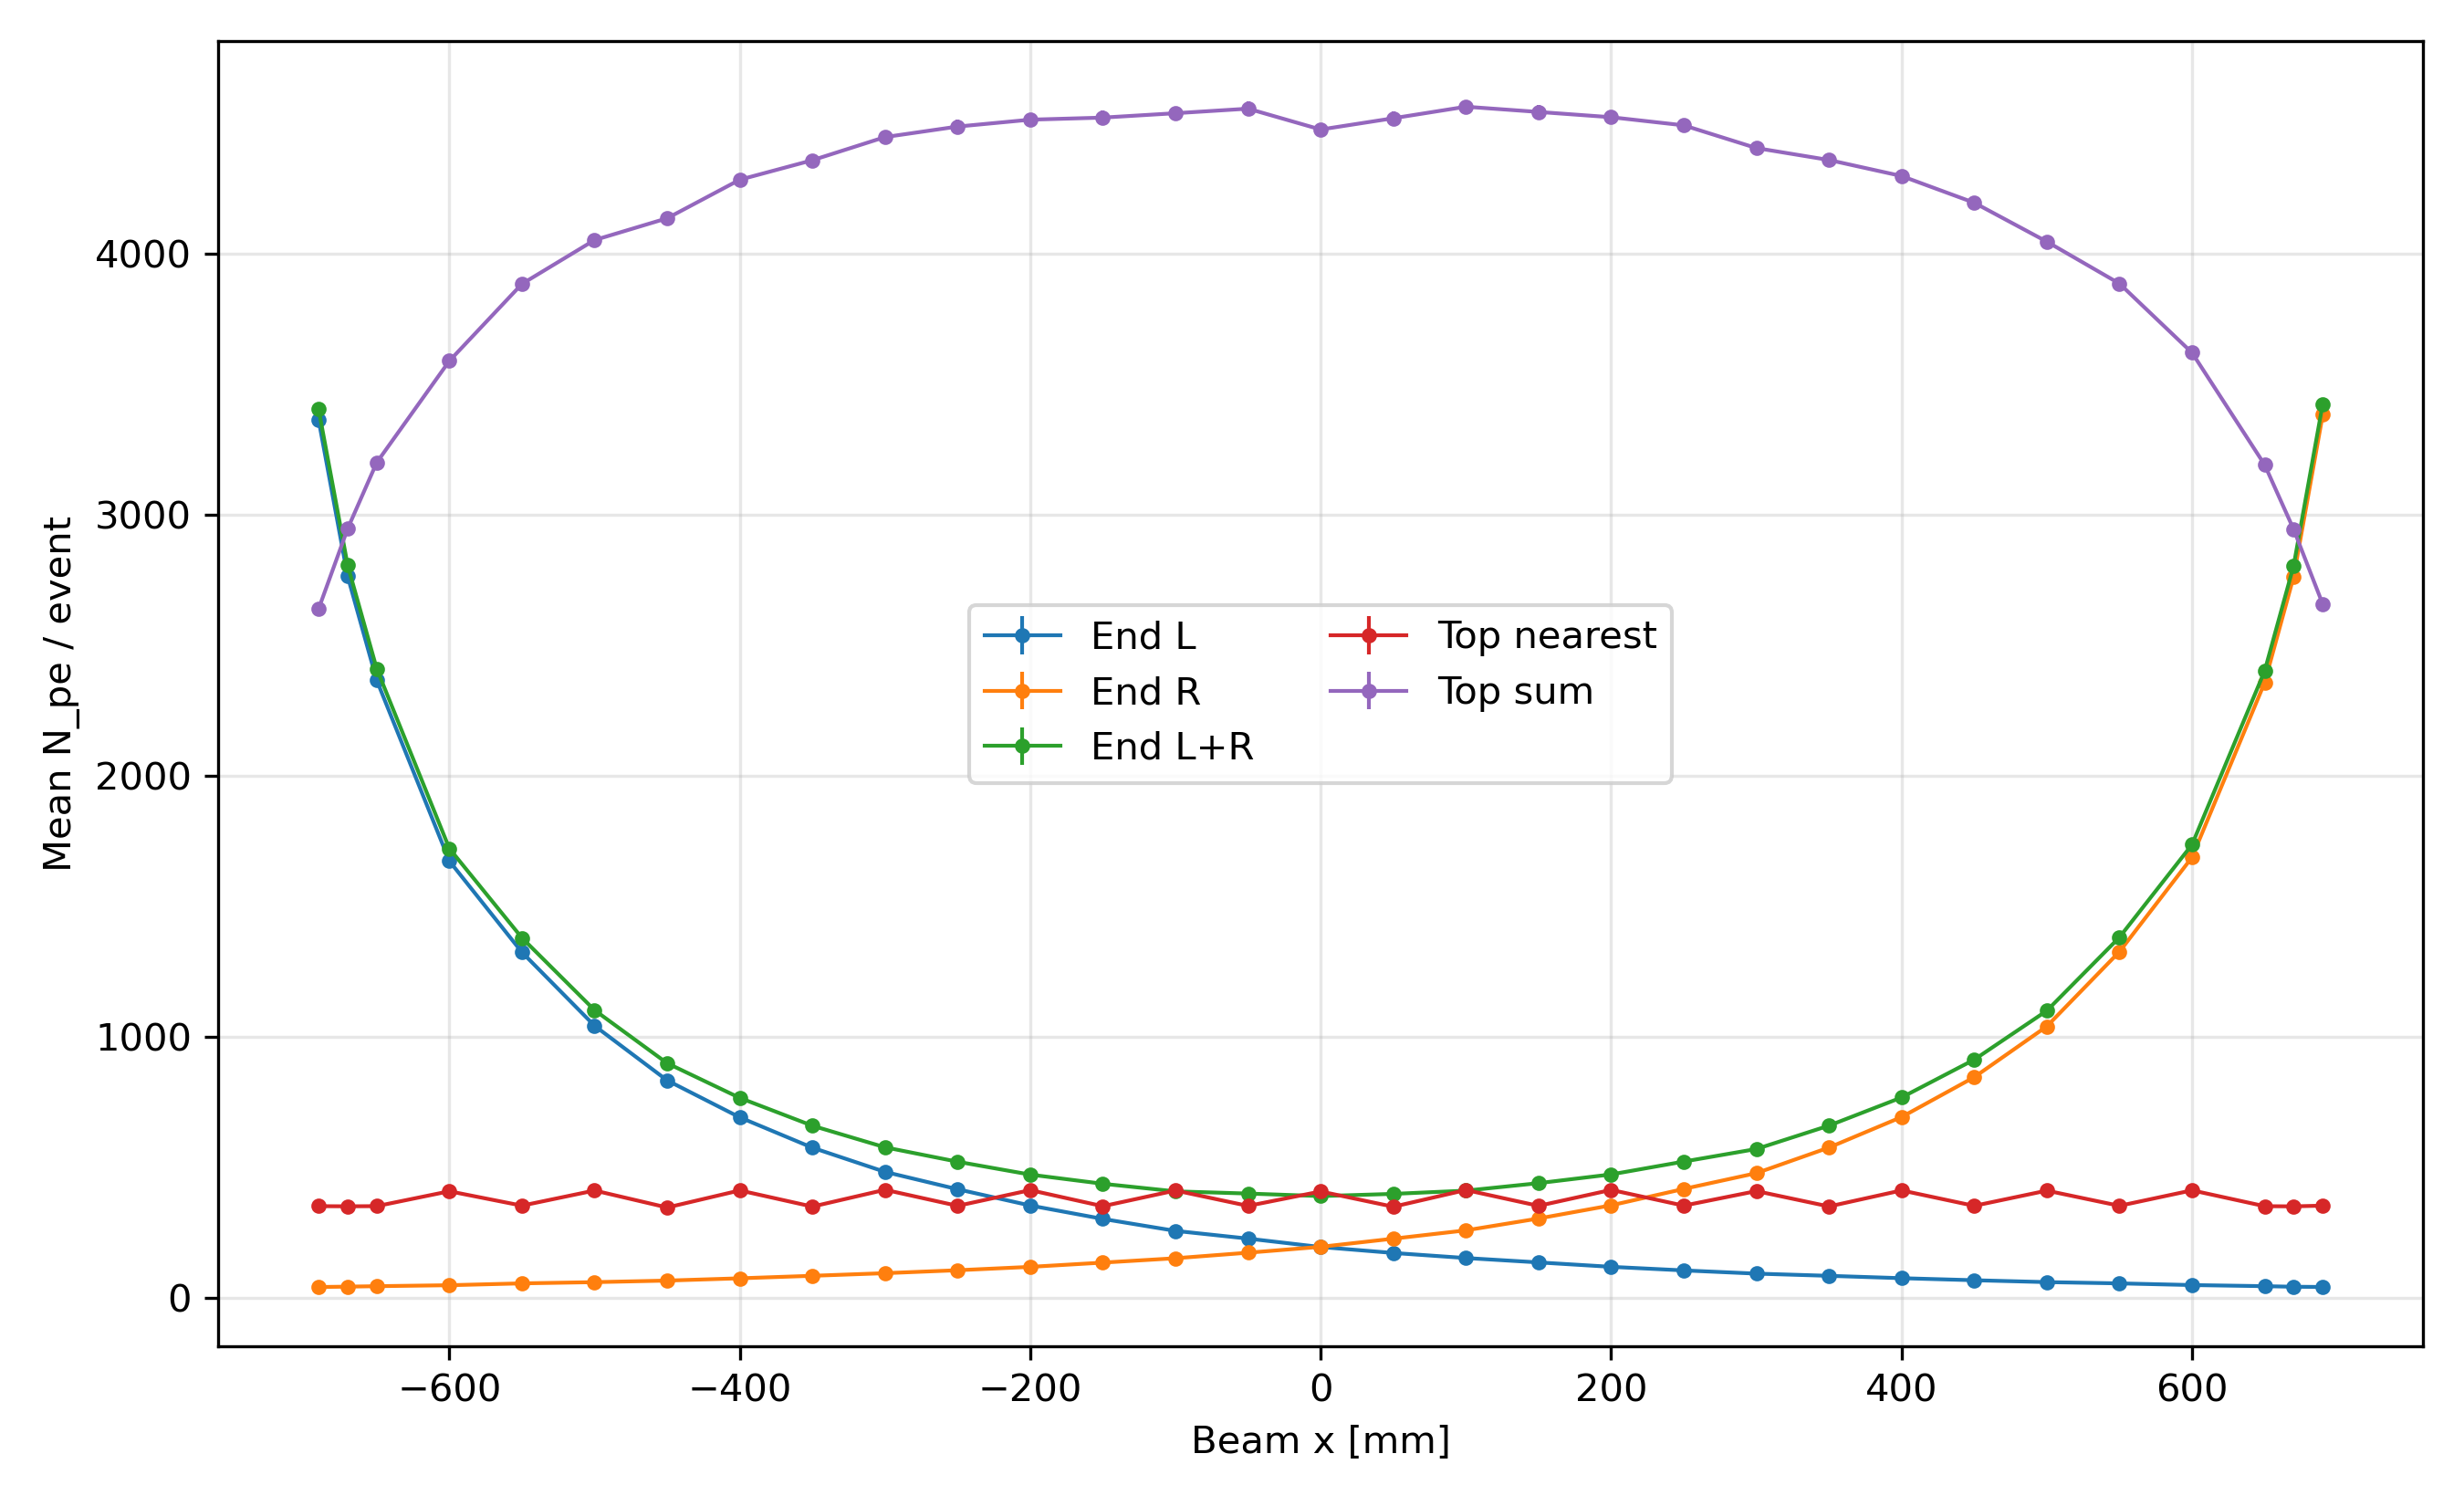
\includegraphics[width=\textwidth,height=0.78\textheight,keepaspectratio]{figs/P1_npe_vs_x.png}
\end{frame}
\begin{frame}{Top localization: full coverage diagonal}
\centering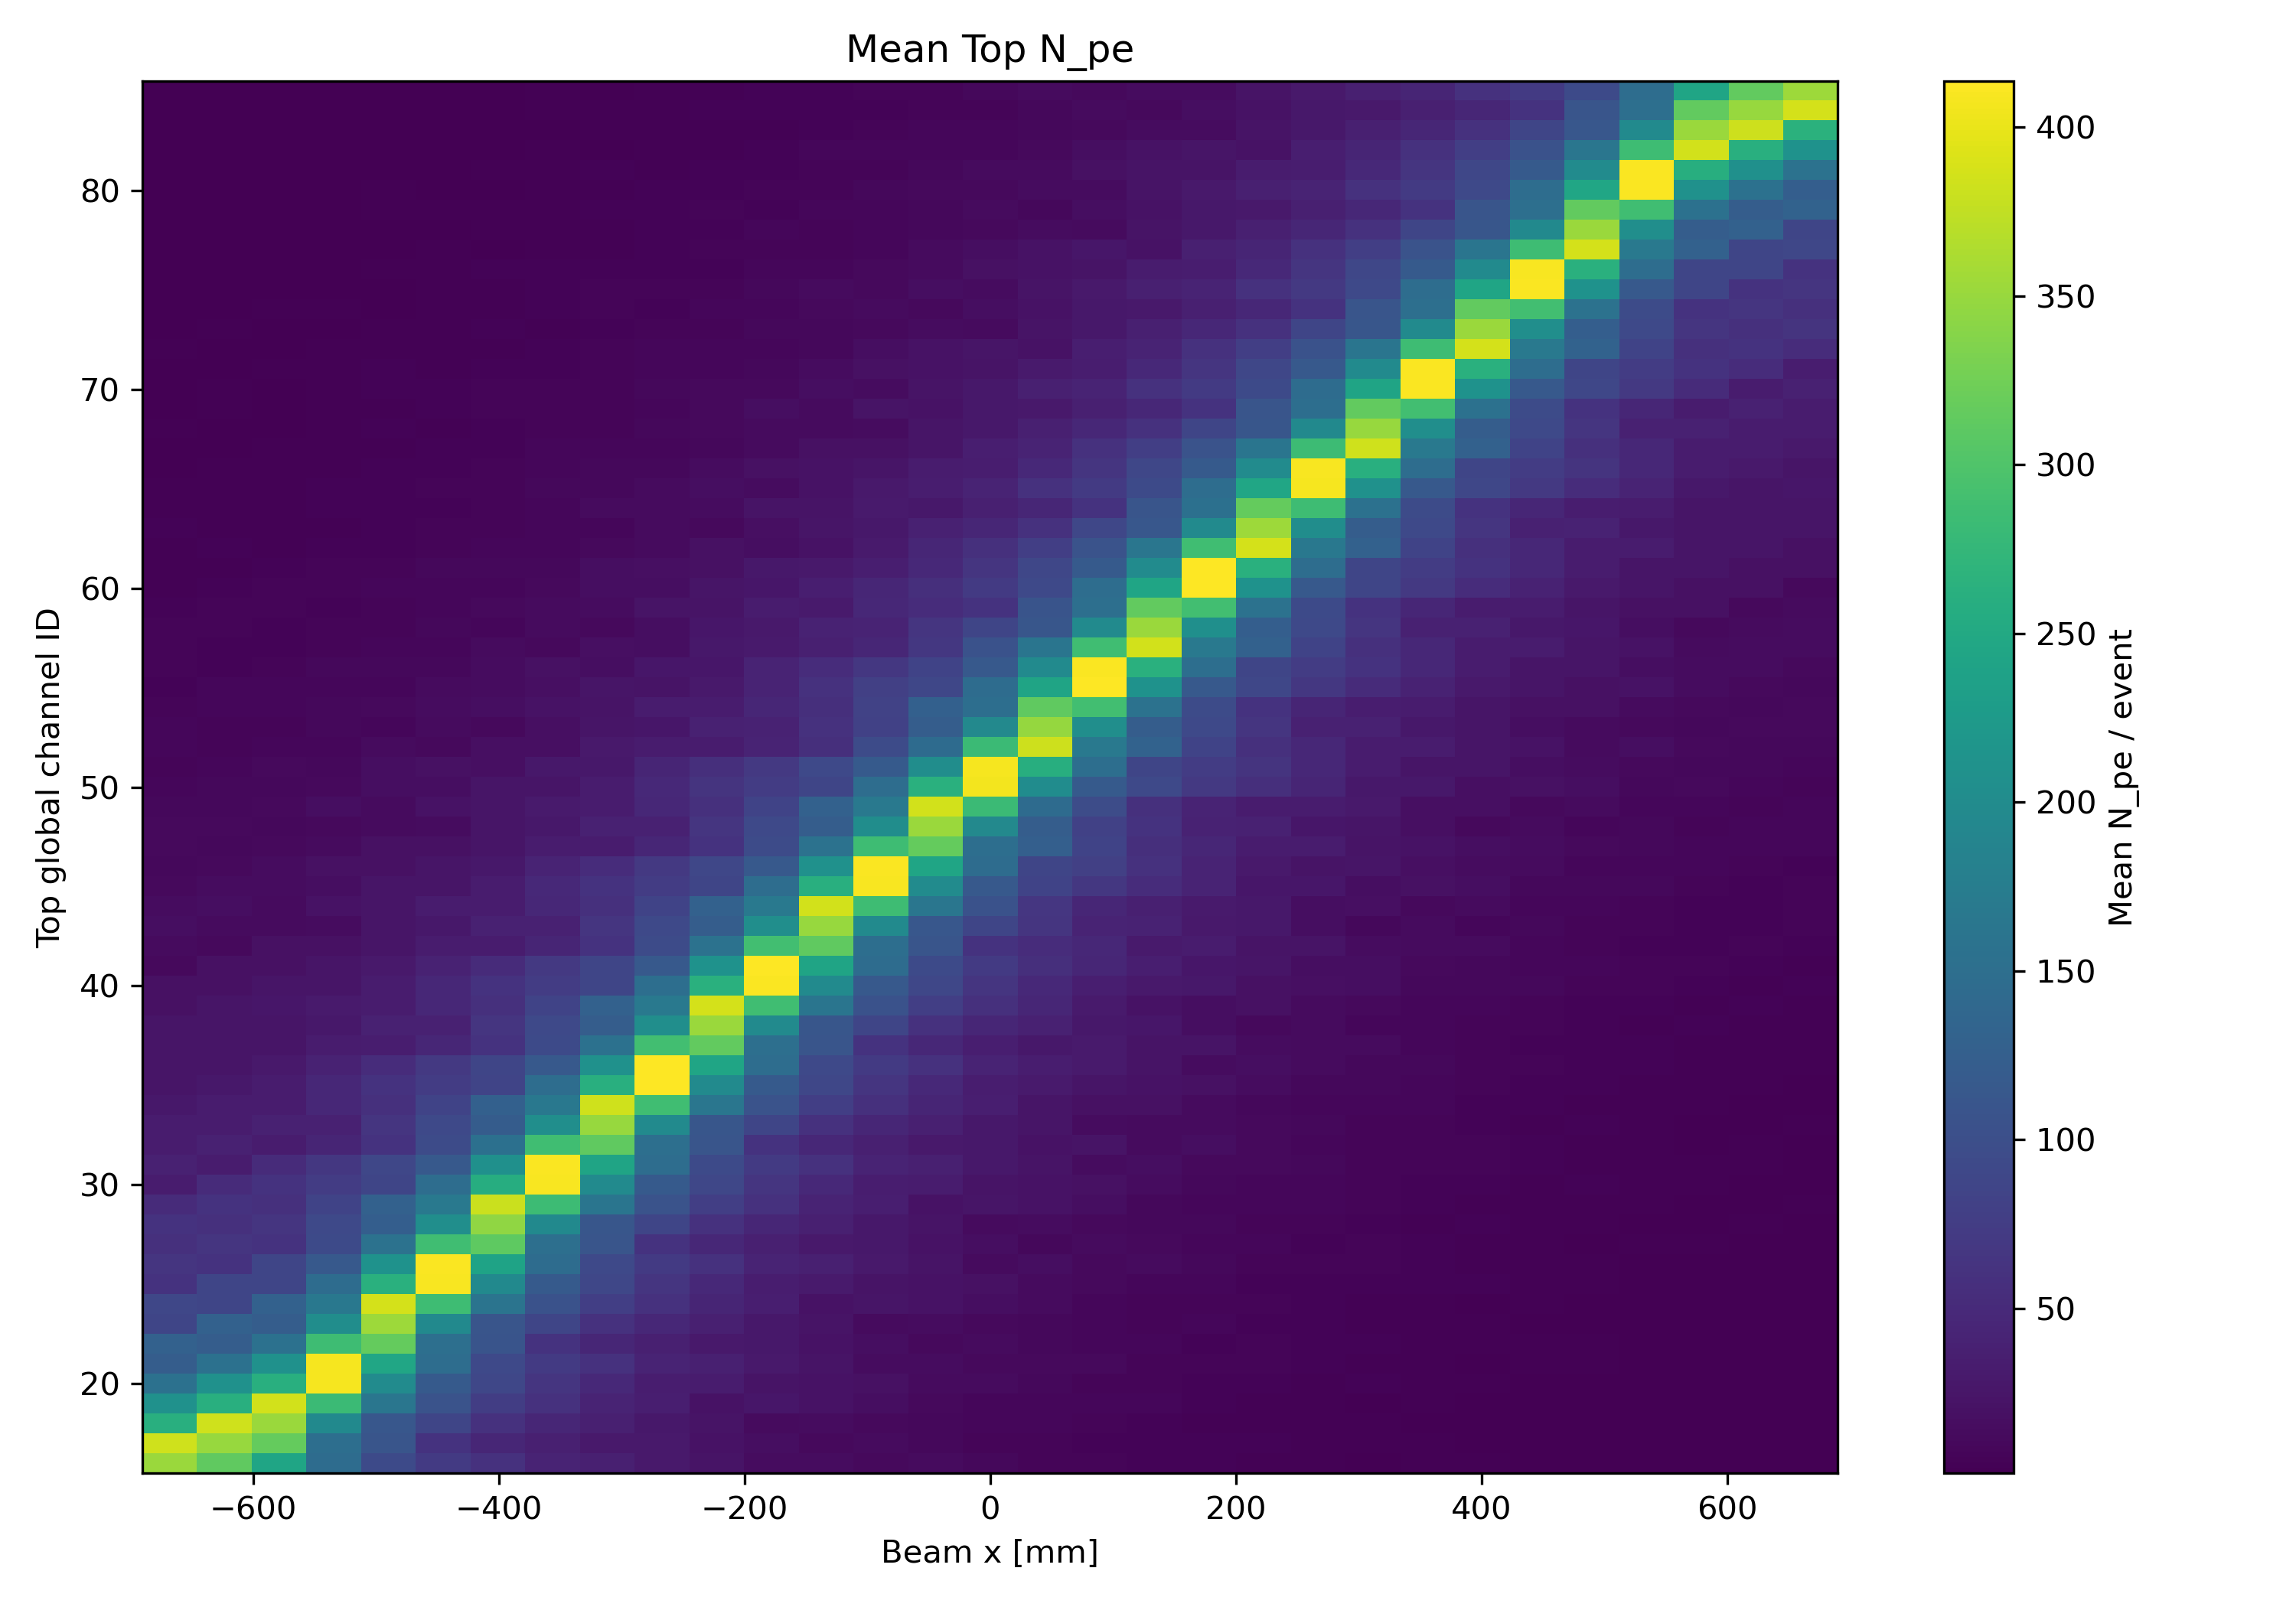
\includegraphics[width=\textwidth,height=0.78\textheight,keepaspectratio]{figs/P2_npe_heatmap_top.png}
\end{frame}
\begin{frame}{Effective attenuation and propagation fits}
\centering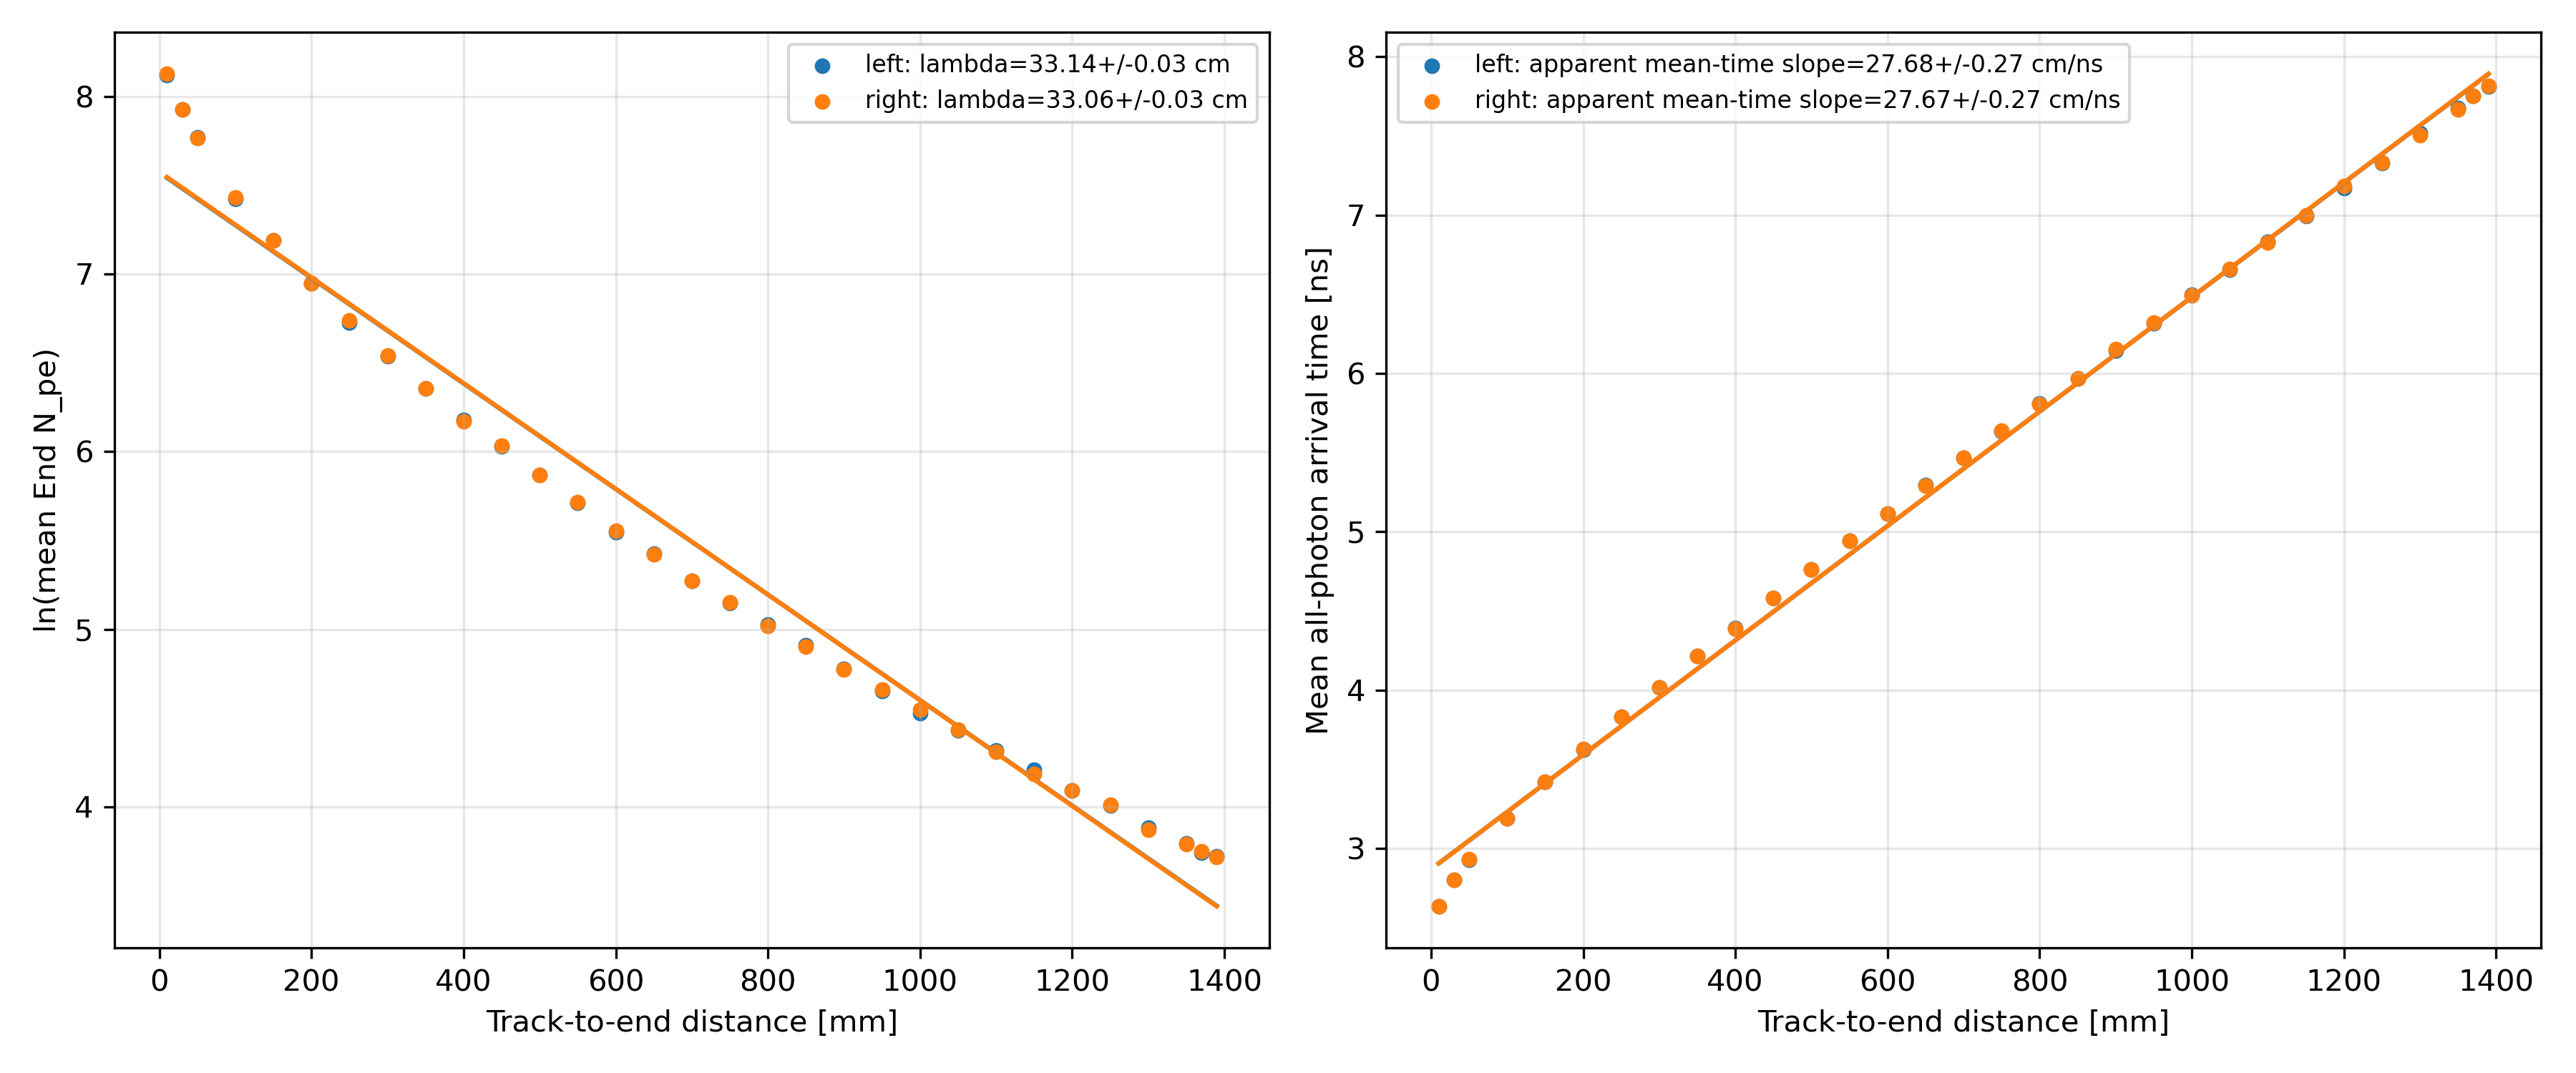
\includegraphics[width=\textwidth,height=0.78\textheight,keepaspectratio]{figs/fits_attenuation_velocity.png}\par\scriptsize $\lambda_{eff,L}=33.14\pm0.03$ cm, $\lambda_{eff,R}=33.06\pm0.03$ cm; $v_{eff}\simeq27.67\pm0.27$ cm/ns. The 160 cm bulk value and $c/n\simeq19$ cm/ns are not fit targets.
\end{frame}
\begin{frame}{Fano-like variance/mean versus x}
\centering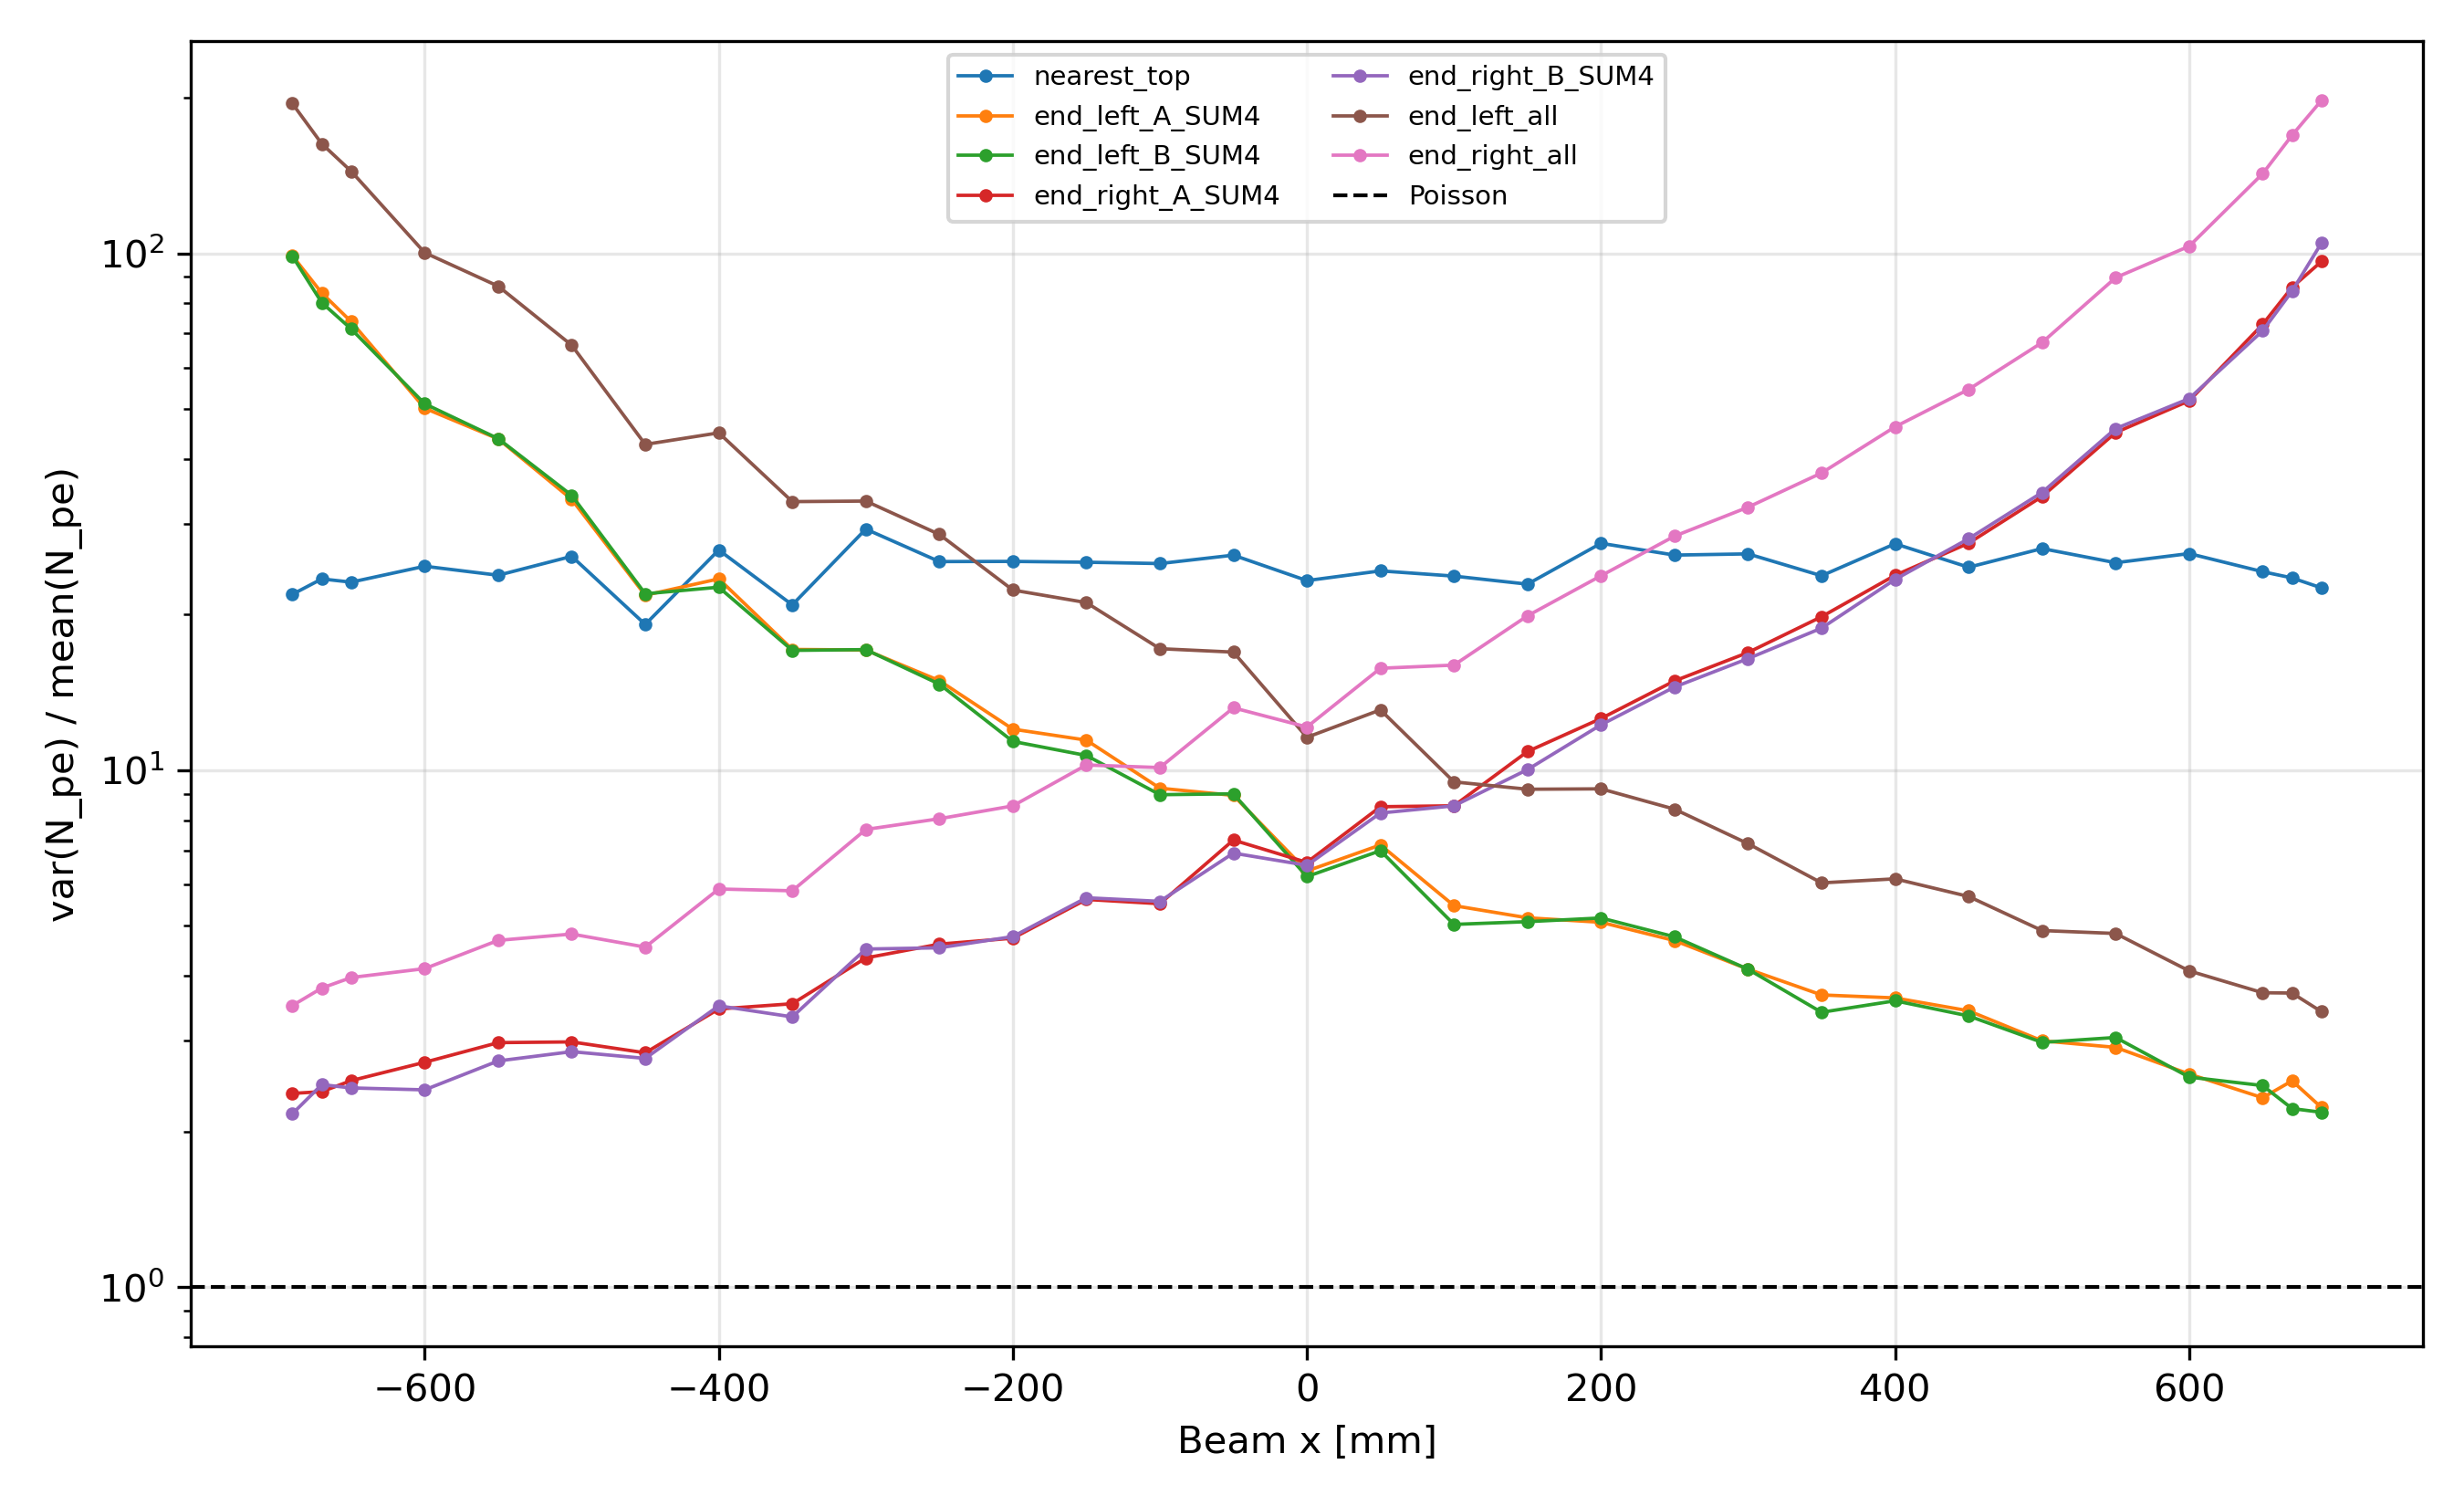
\includegraphics[width=\textwidth,height=0.78\textheight,keepaspectratio]{figs/P3_fano_vs_x.png}
\end{frame}
\begin{frame}{Poisson and Gaussian tail example}
\centering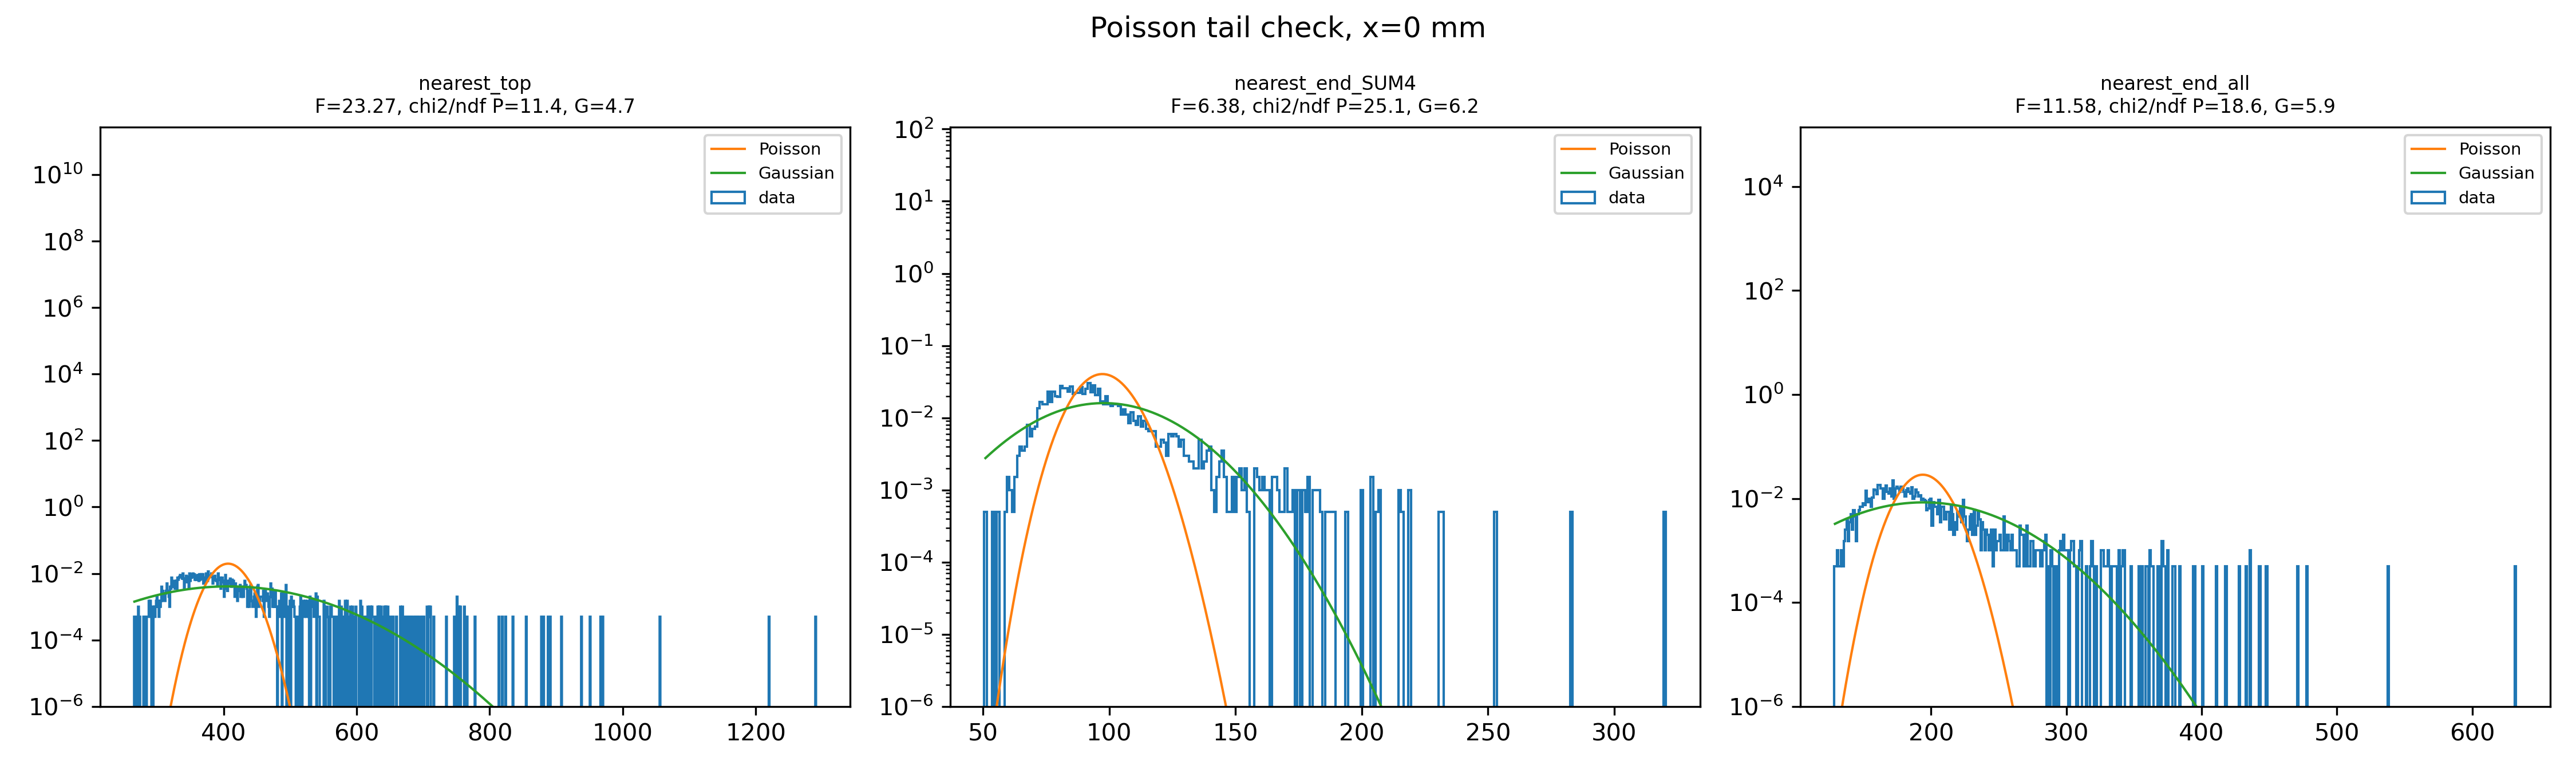
\includegraphics[width=\textwidth,height=0.78\textheight,keepaspectratio]{figs/P4_poisson_check_x0.png}
\end{frame}
\begin{frame}{Arrival-time examples: all photons and FPT}
\centering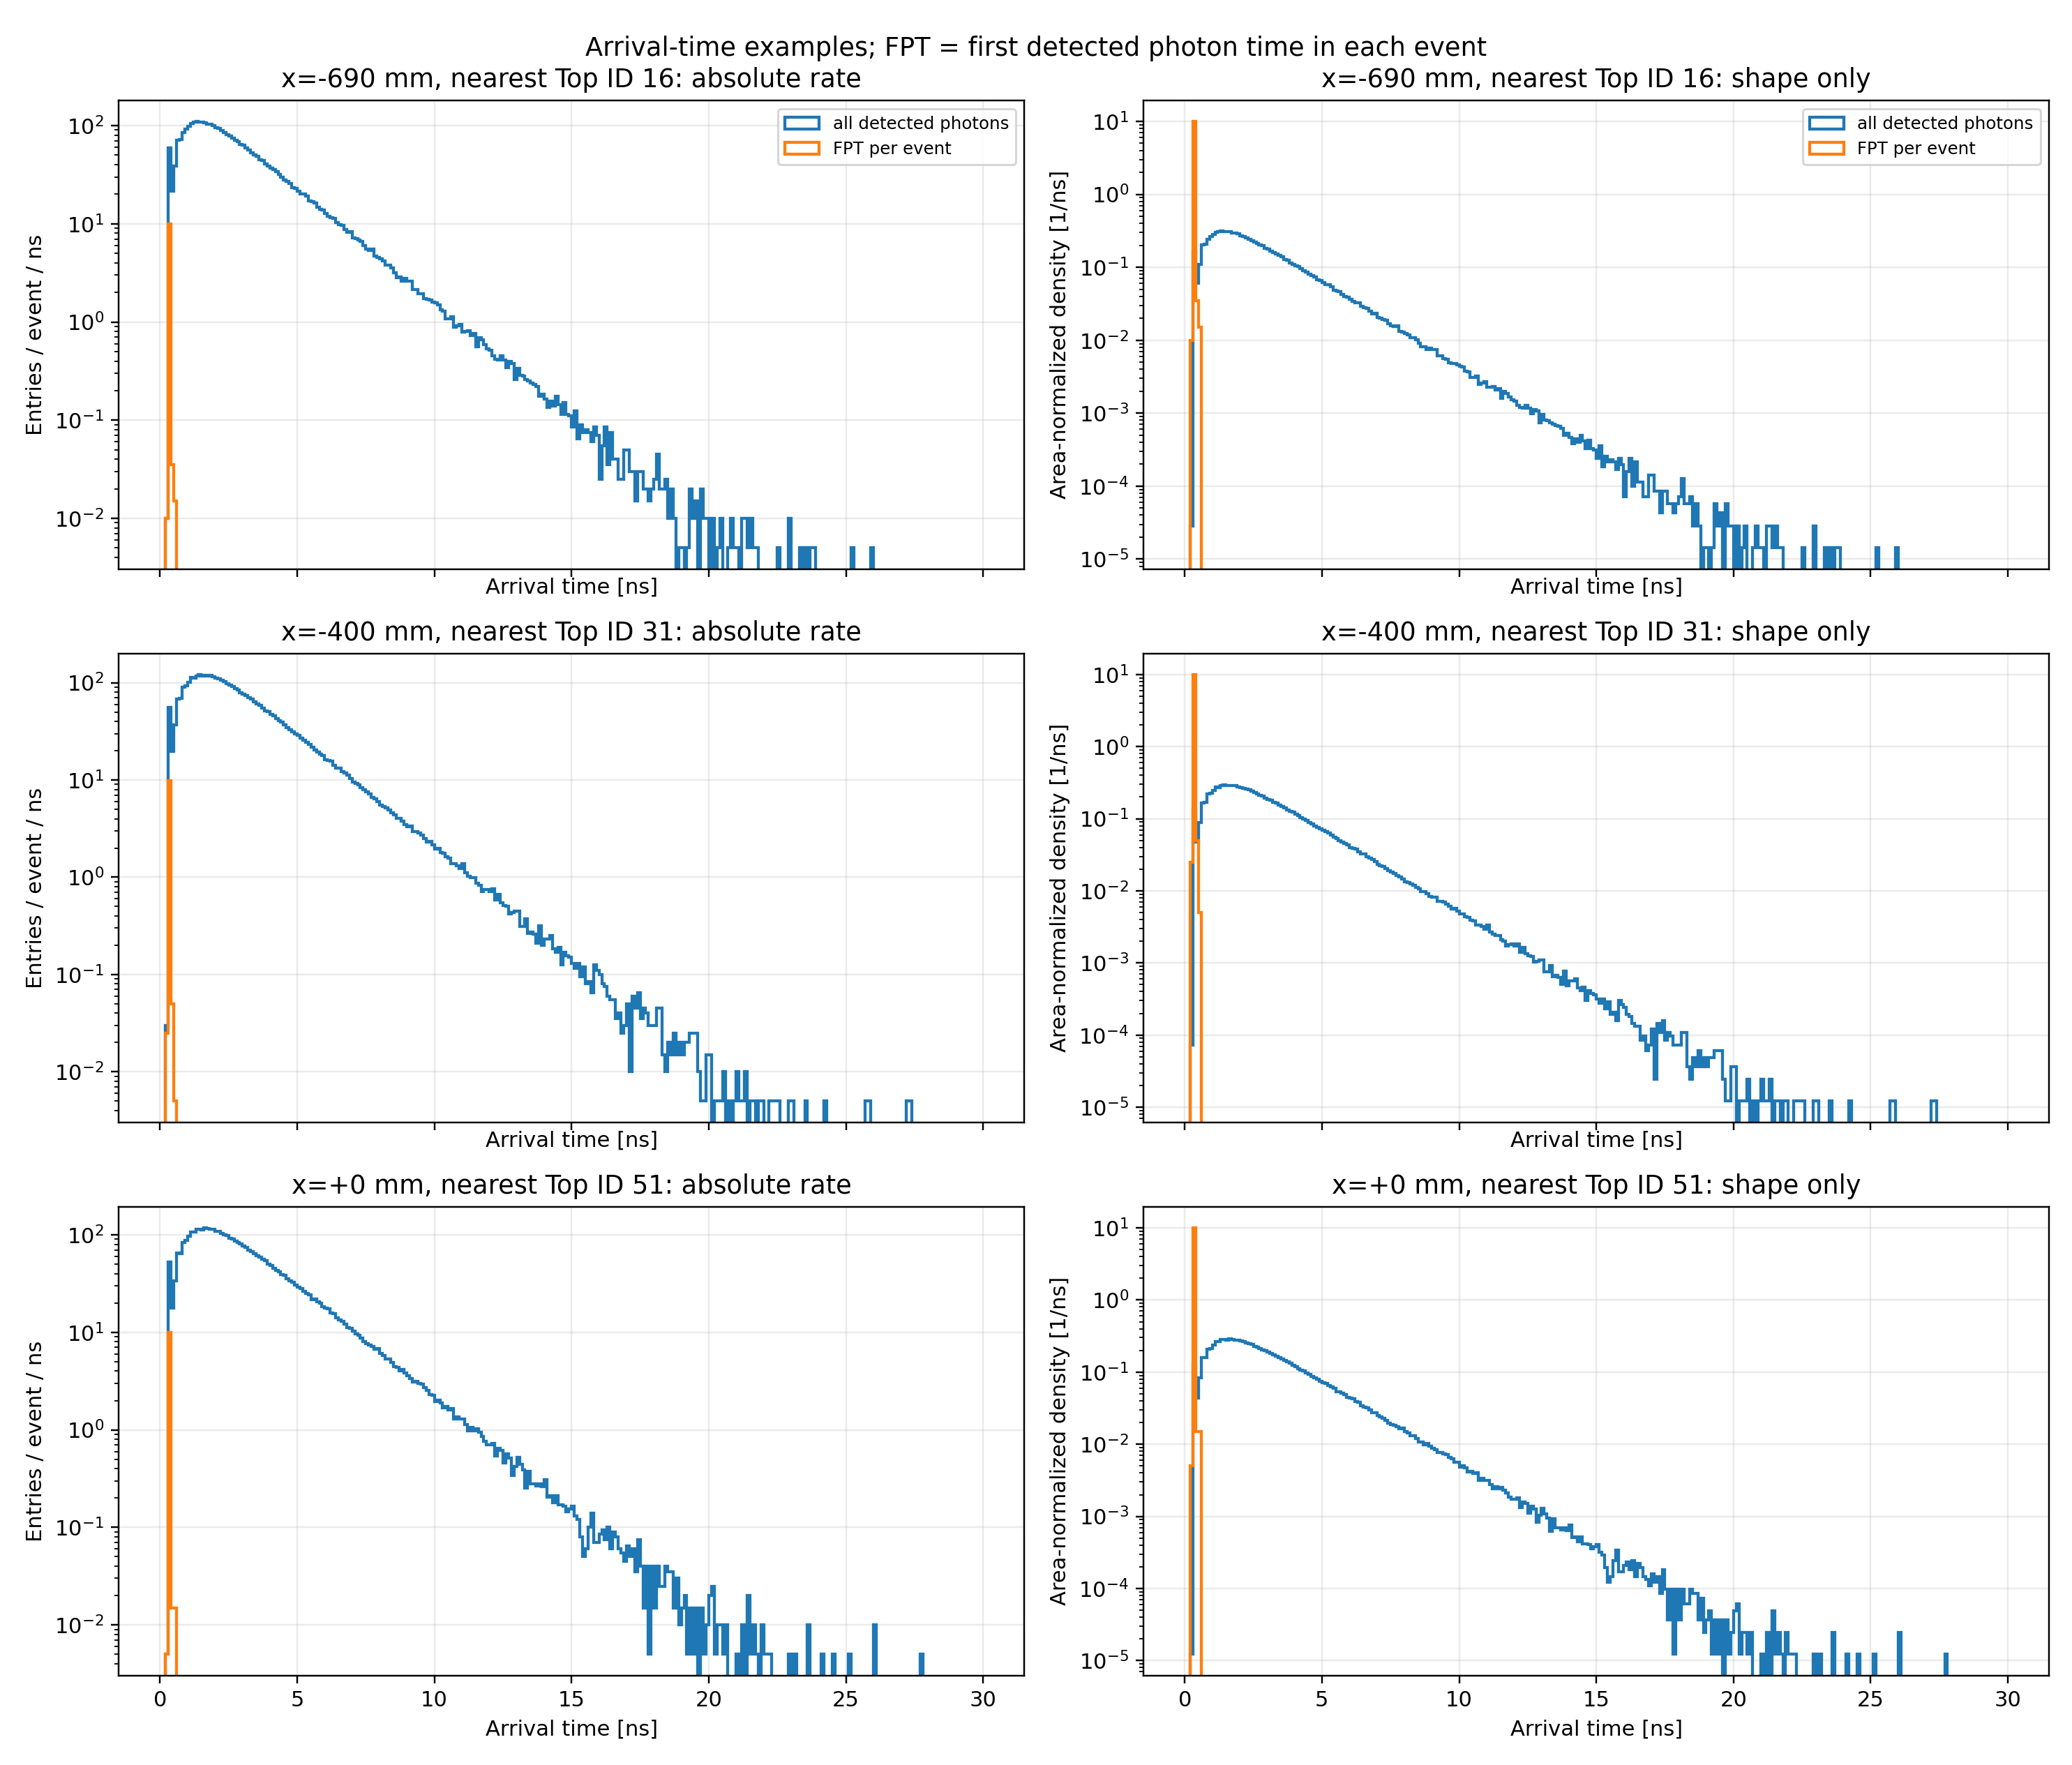
\includegraphics[width=\textwidth,height=0.78\textheight,keepaspectratio]{figs/P5_tdist_examples.png}
\end{frame}
\begin{frame}{Mean arrival time and FPT versus x}
\centering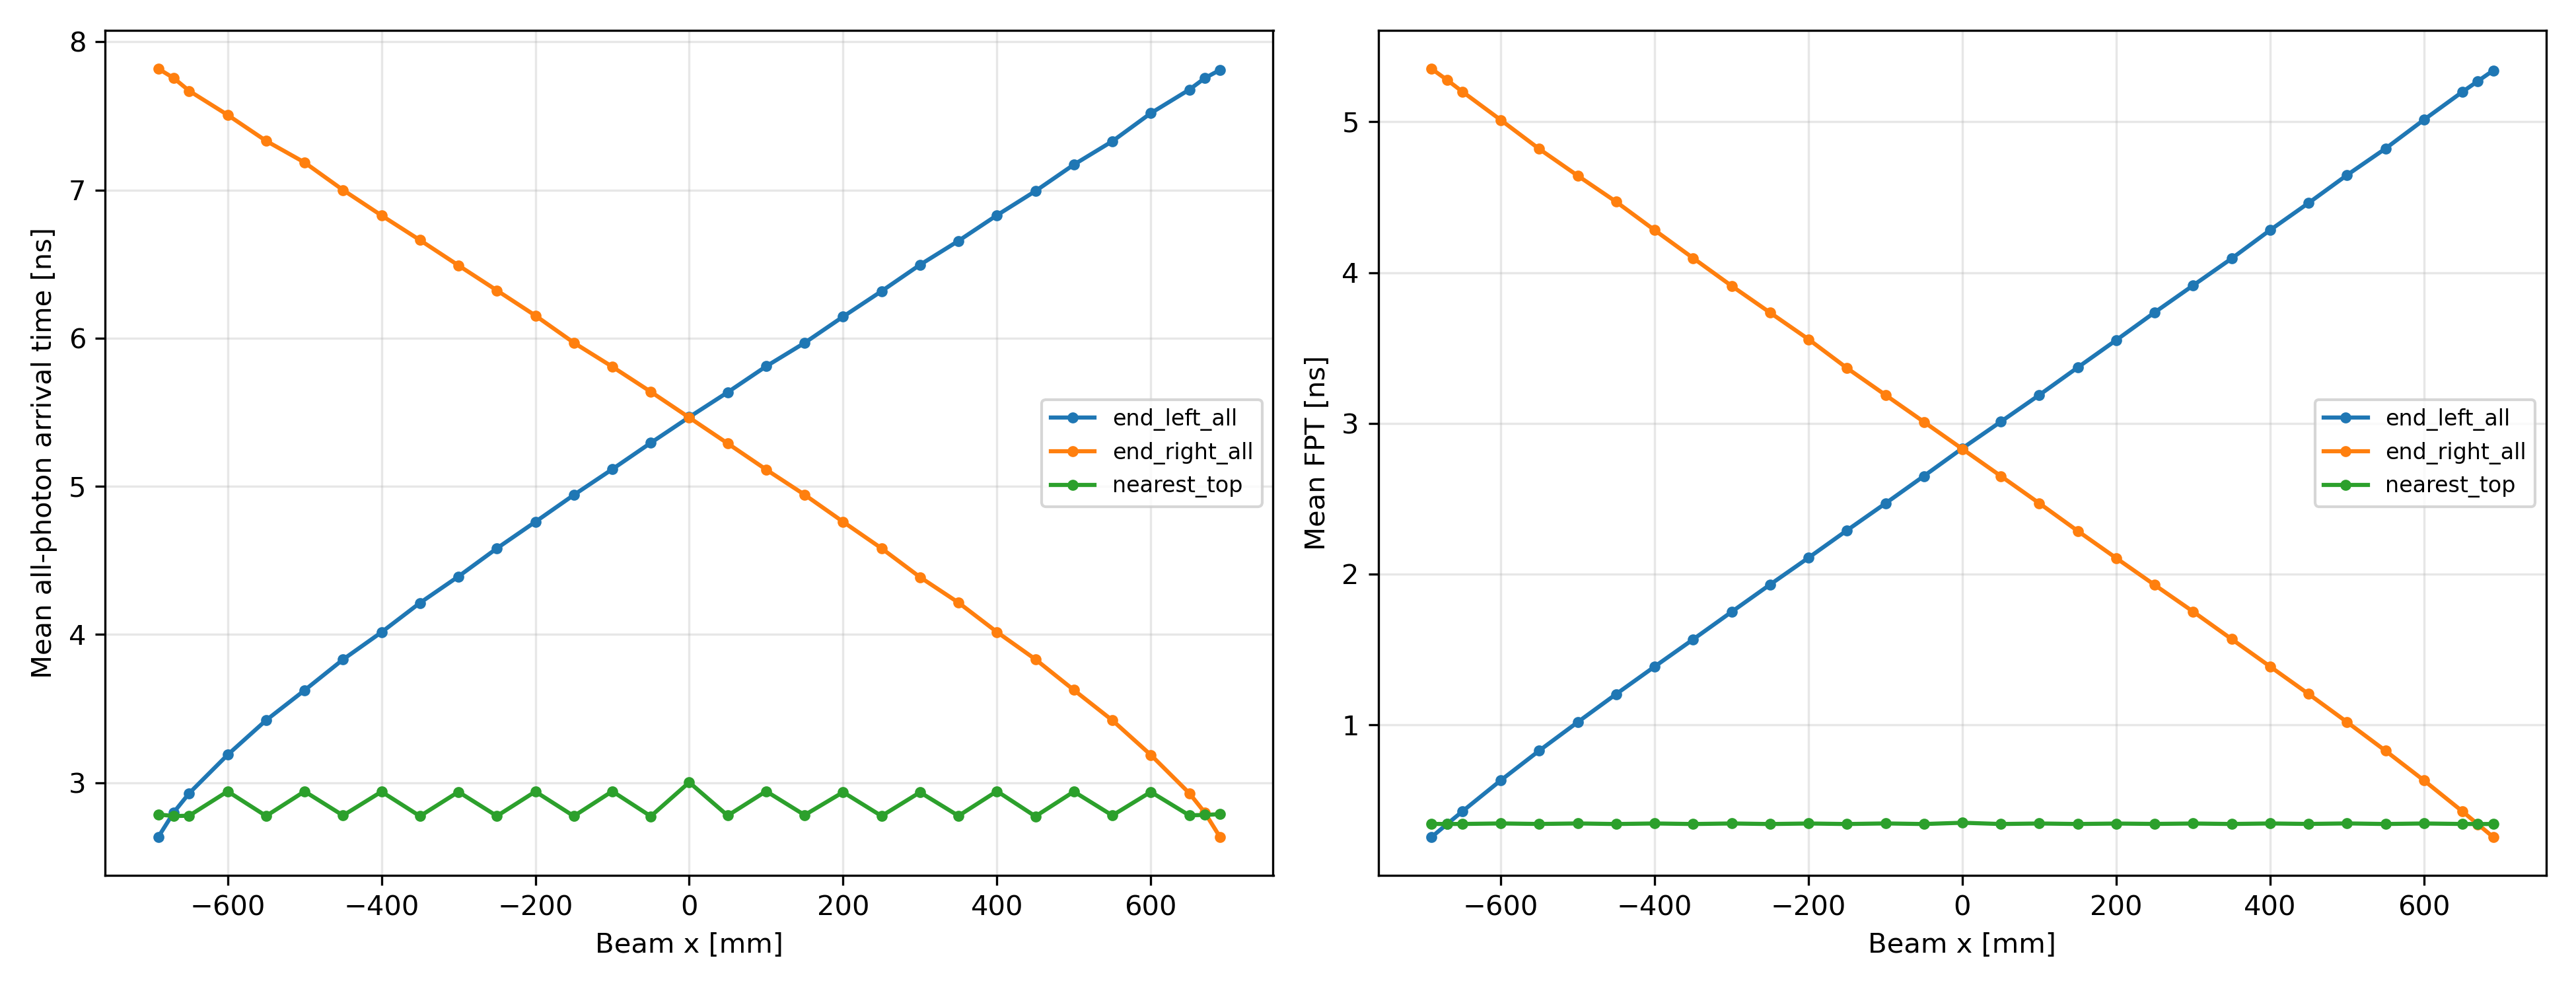
\includegraphics[width=\textwidth,height=0.78\textheight,keepaspectratio]{figs/P6_tmean_vs_x.png}
\end{frame}
\section{Window effect and timing}
\begin{frame}{Window-track collection effect: five-run test}

\begin{columns}[T]\column{0.47\textwidth}
\scriptsize\resizebox{\textwidth}{!}{\begin{tabular}{lrr}\toprule
Run & contrast [Npe] & significance \\ \midrule
Existing -650 & $34.60\pm2.94$ & $11.78$ \\
A -652 center & $2.86\pm2.65$ & $1.08$ \\
B -642 midpoint & $-0.33\pm3.35$ & $-0.10$ \\
C1 -648 (+4 mm) & $21.08\pm3.20$ & $6.59$ \\
C2 -654 mirror & $34.38\pm2.95$ & $11.64$ \\
\bottomrule\end{tabular}}
\column{0.51\textwidth}
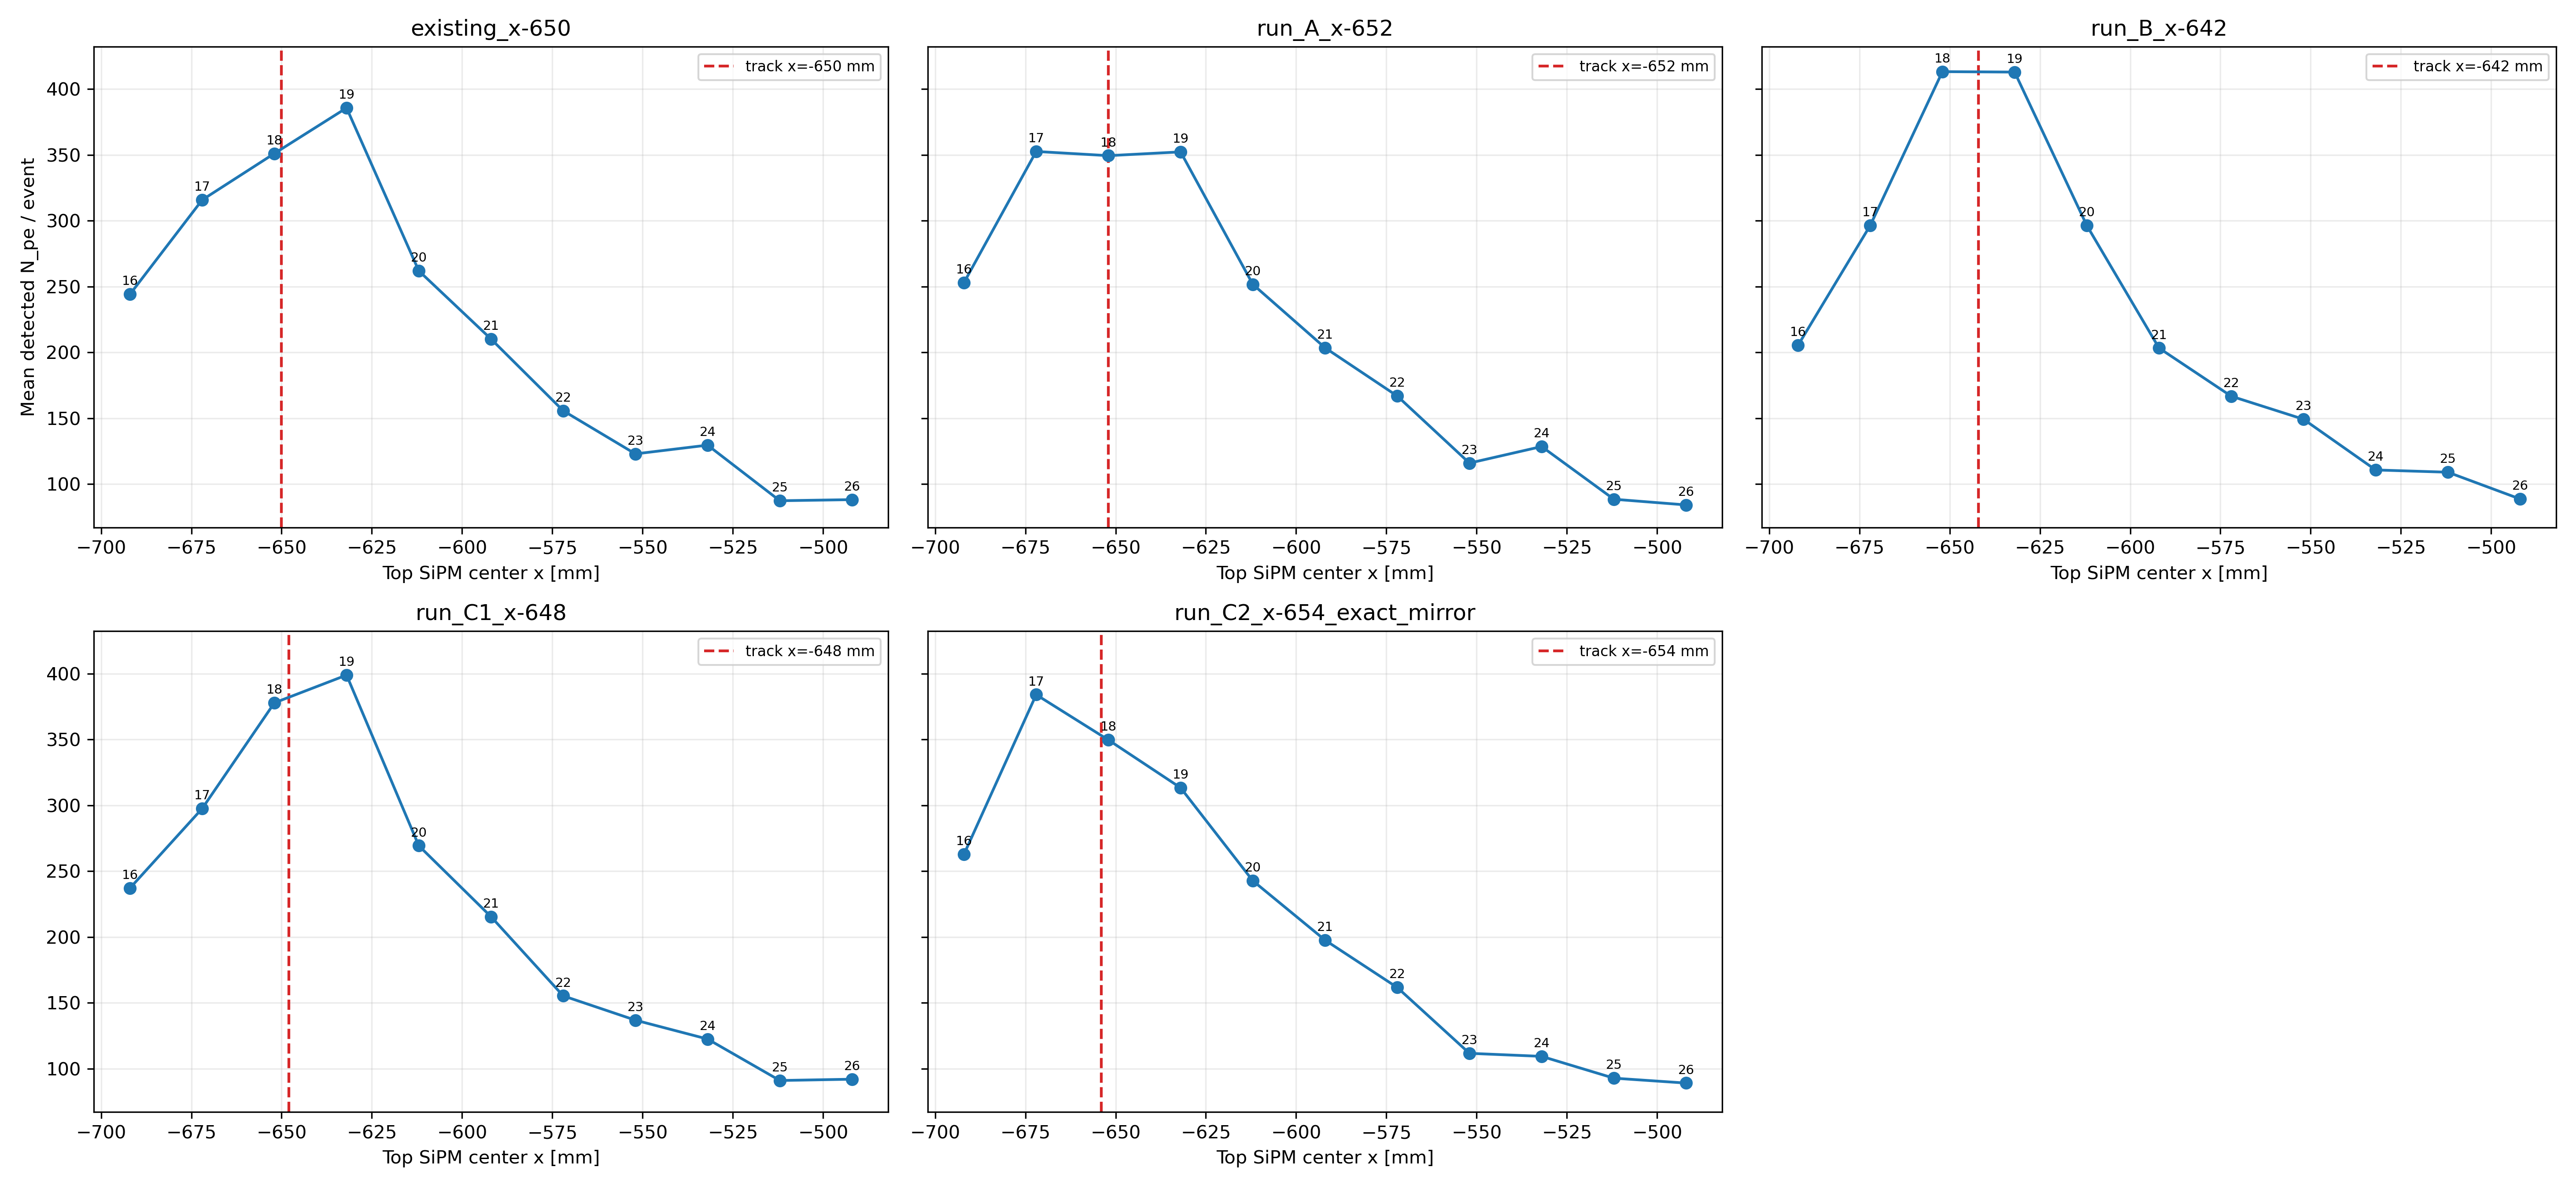
\includegraphics[width=\textwidth]{figs/exec08b_window_dip_profiles.png}
\end{columns}
\begin{block}{Finding}
Local symmetric $\pm2$ mm effect: about 9.8\% at about 12 sigma; null when centered
and at midpoint. The scan and channel map remain valid.
\end{block}

\end{frame}
\begin{frame}{Intrinsic End SUM4 timing}
\centering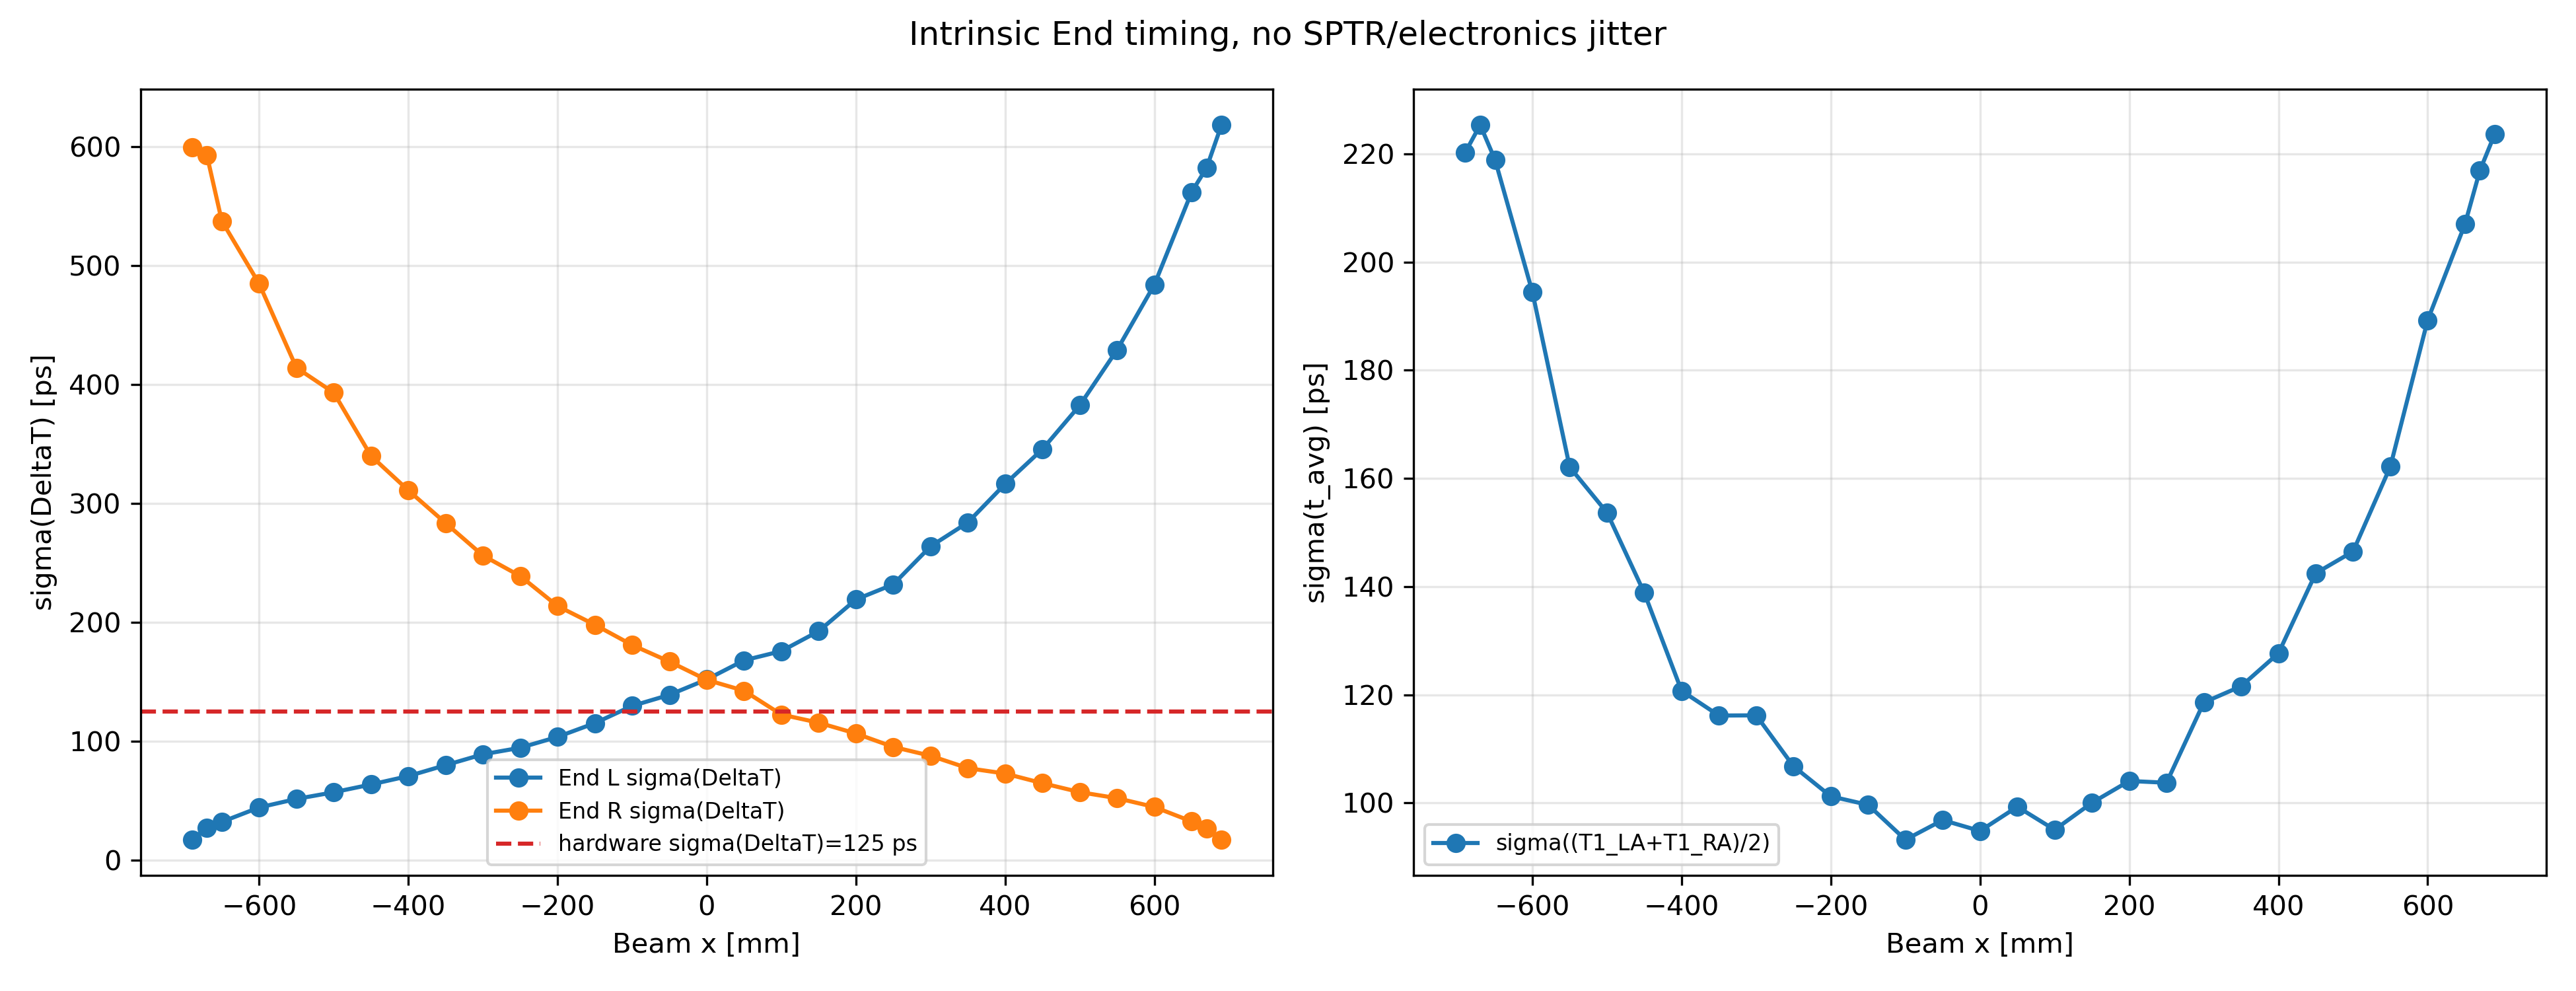
\includegraphics[width=\textwidth,height=0.78\textheight,keepaspectratio]{figs/P7_deltaT_end.png}\par\scriptsize $\sigma_{group}=\sigma(\Delta T_{AB})/\sqrt{2}$; no SPTR/jitter. The 88 ps hardware context is not directly comparable.
\end{frame}
\begin{frame}{Timing gate lifted: narrower EndTop is physical}

\begin{columns}[T]\column{0.48\textwidth}
\scriptsize\resizebox{\textwidth}{!}{\begin{tabular}{rrrrr}\toprule
$x$ & side & EndTop [ps] & End-only [ps] & ratio \\ \midrule
-400 & L & $50.0\pm0.8$ & $66.1\pm0.5$ & $0.756\pm0.013$ \\
-400 & R & $219.9\pm3.5$ & $248.4\pm1.8$ & $0.885\pm0.015$ \\
+0 & L & $107.5\pm1.7$ & $131.4\pm0.9$ & $0.818\pm0.014$ \\
+0 & R & $107.2\pm1.7$ & $129.5\pm0.9$ & $0.828\pm0.014$ \\
+400 & L & $223.8\pm3.5$ & $247.5\pm1.8$ & $0.904\pm0.016$ \\
+400 & R & $51.5\pm0.8$ & $65.9\pm0.5$ & $0.781\pm0.014$ \\
\bottomrule\end{tabular}}
\column{0.50\textwidth}
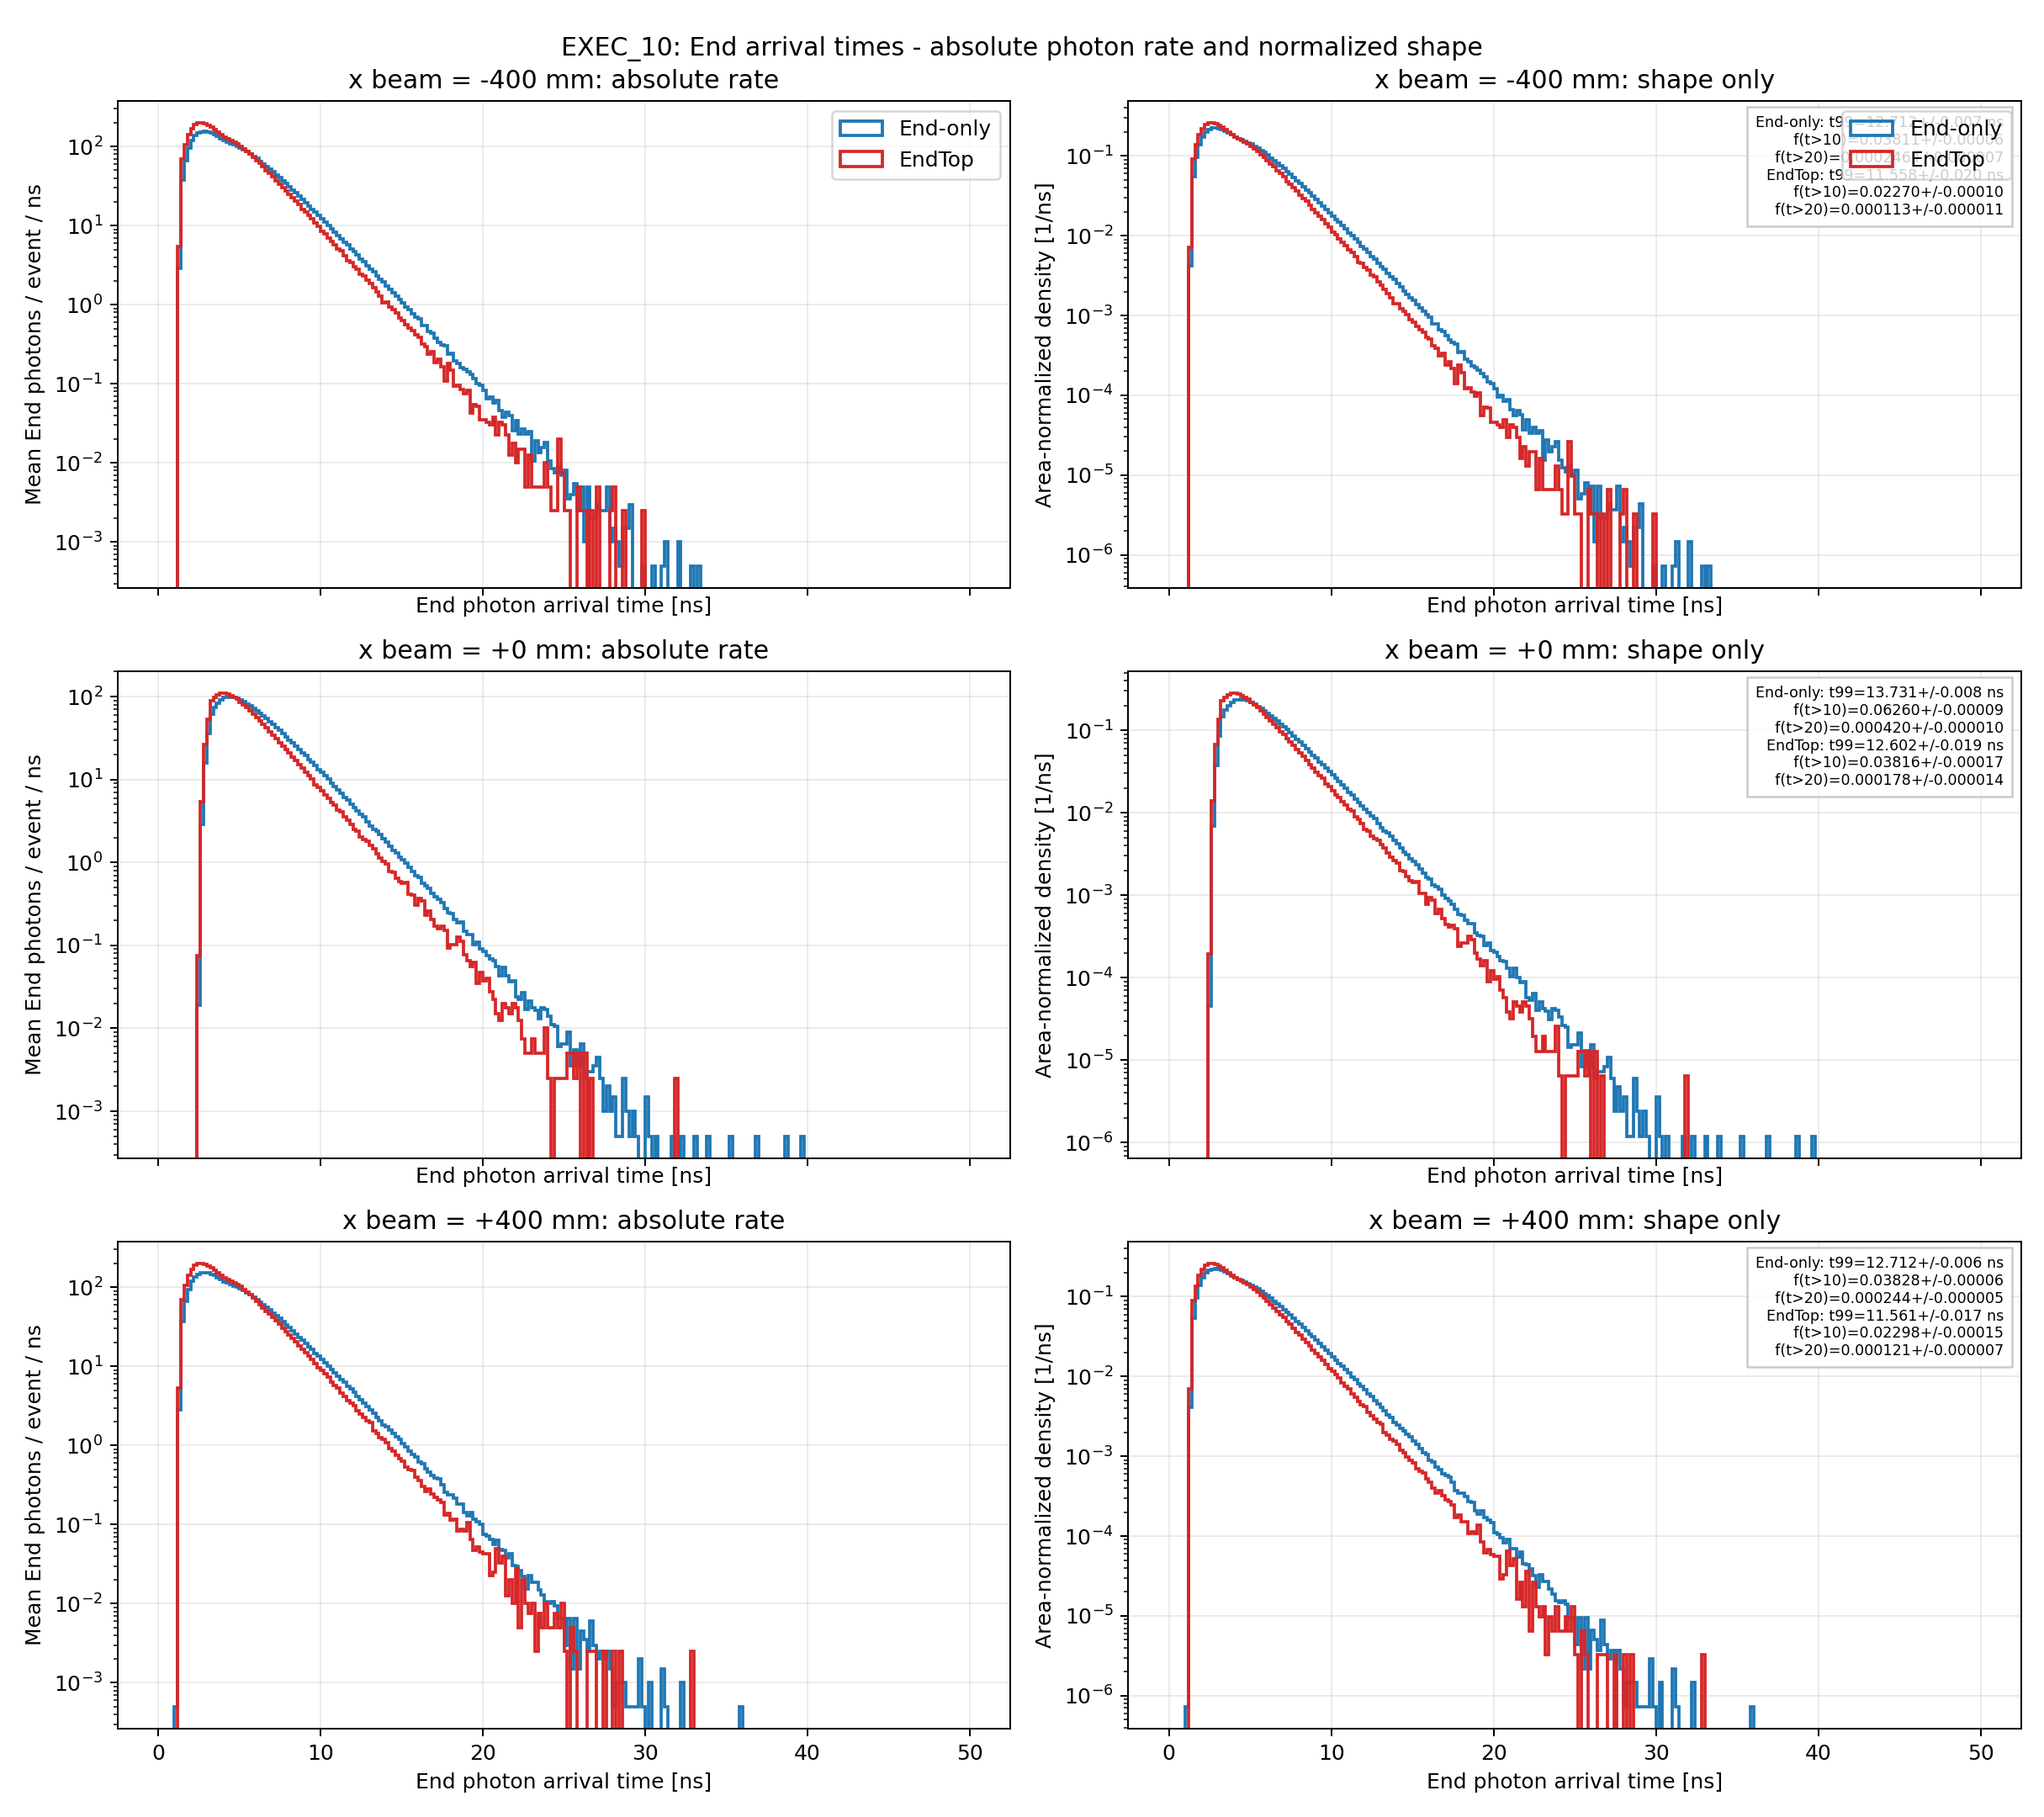
\includegraphics[width=\textwidth]{figs/exec09_tail_comparison.png}
\end{columns}
\begin{alertblock}{Confirmed mechanism}
Across $x=0,\pm400$ mm, EndTop lowers $t99$ by
1.14 ns and suppresses late fractions
at more than 10.3 sigma.
\end{alertblock}

\end{frame}
\begin{frame}{Top readout: analytic timing estimate only}

\centering\small
\begin{tabular}{rrr}\toprule
$x$ [mm] & nearest Top $N_{pe}$ & $\sigma_{t,est}$ [ps] \\ \midrule
-690 & $350.9\pm2.0$ & $59.92\pm0.17$ \\
-650 & $351.0\pm2.0$ & $59.91\pm0.17$ \\
-400 & $411.3\pm2.3$ & $55.35\pm0.16$ \\
+0 & $407.3\pm2.2$ & $55.62\pm0.15$ \\
+400 & $411.4\pm2.4$ & $55.34\pm0.16$ \\
+650 & $350.9\pm2.1$ & $59.93\pm0.18$ \\
+690 & $353.0\pm2.0$ & $59.75\pm0.17$ \\
\bottomrule\end{tabular}
\vspace{0.35cm}
\begin{block}{Definition and scope}
$\sigma_{t,est}=\sqrt{0.7\,\mathrm{ns}\times1.8\,\mathrm{ns}}/\sqrt{N_{pe}}
=1.122\,\mathrm{ns}/\sqrt{N_{pe}}$. This is an analytic orientation,
not a simulated timing resolution; Top has no test-beam counterpart.
\end{block}

\end{frame}
\begin{frame}{Numerical conclusions}

\small\begin{itemize}
 \item At center: End sum $389.6\pm2.1$, nearest Top $407.3\pm2.2$;
       at $x=-690$ mm: End sum $3404.2\pm18.3$, nearest Top $350.9\pm2.0$.
 \item $\lambda_{eff}$: L $33.14\pm0.03$ cm,
       R $33.06\pm0.03$ cm;
       $v_{eff}$: about $27.67\pm0.27$ cm/ns.
 \item Nearest-Top var/mean: median 24.81, range
       19.14--29.27;
       data are strongly over-dispersed relative to Poisson.
 \item Intrinsic End $\sigma_{group}$: mean 148.3 ps,
       range 12.1--437.3 ps.
 \item EndTop/End-only timing ratio: $0.756\pm0.016$
       to $0.904\pm0.016$.
 \item Three findings: window-track dip characterized; late-tail drain confirmed;
       complete 86-channel coverage and localization gate validated.
\end{itemize}

\end{frame}
\appendix
\begin{frame}{Backup: validation and gates}

\begin{itemize}
 \item 31/31 ROOT files pass: event IDs 0--1999, matching beam x, aggregate IDs 0--85.
 \item Top localization passes all positions: strict nearest maximum except the documented
       $x\equiv10\pmod{20}$ window-track effect (maximum among nearest two, deficit below 15\%).
 \item At x=300 mm the two candidates differ by only 0.08 sigma and pass as a statistical tie.
 \item MPT checks pass: RINDEX 1.58, yield 10400/MeV, decay 1.8 ns, rise 0.7 ns,
       ABSLENGTH 160 cm, emission peak 408.8 nm.
\end{itemize}

\end{frame}
\begin{frame}{Backup: ID18 impact maps}
\centering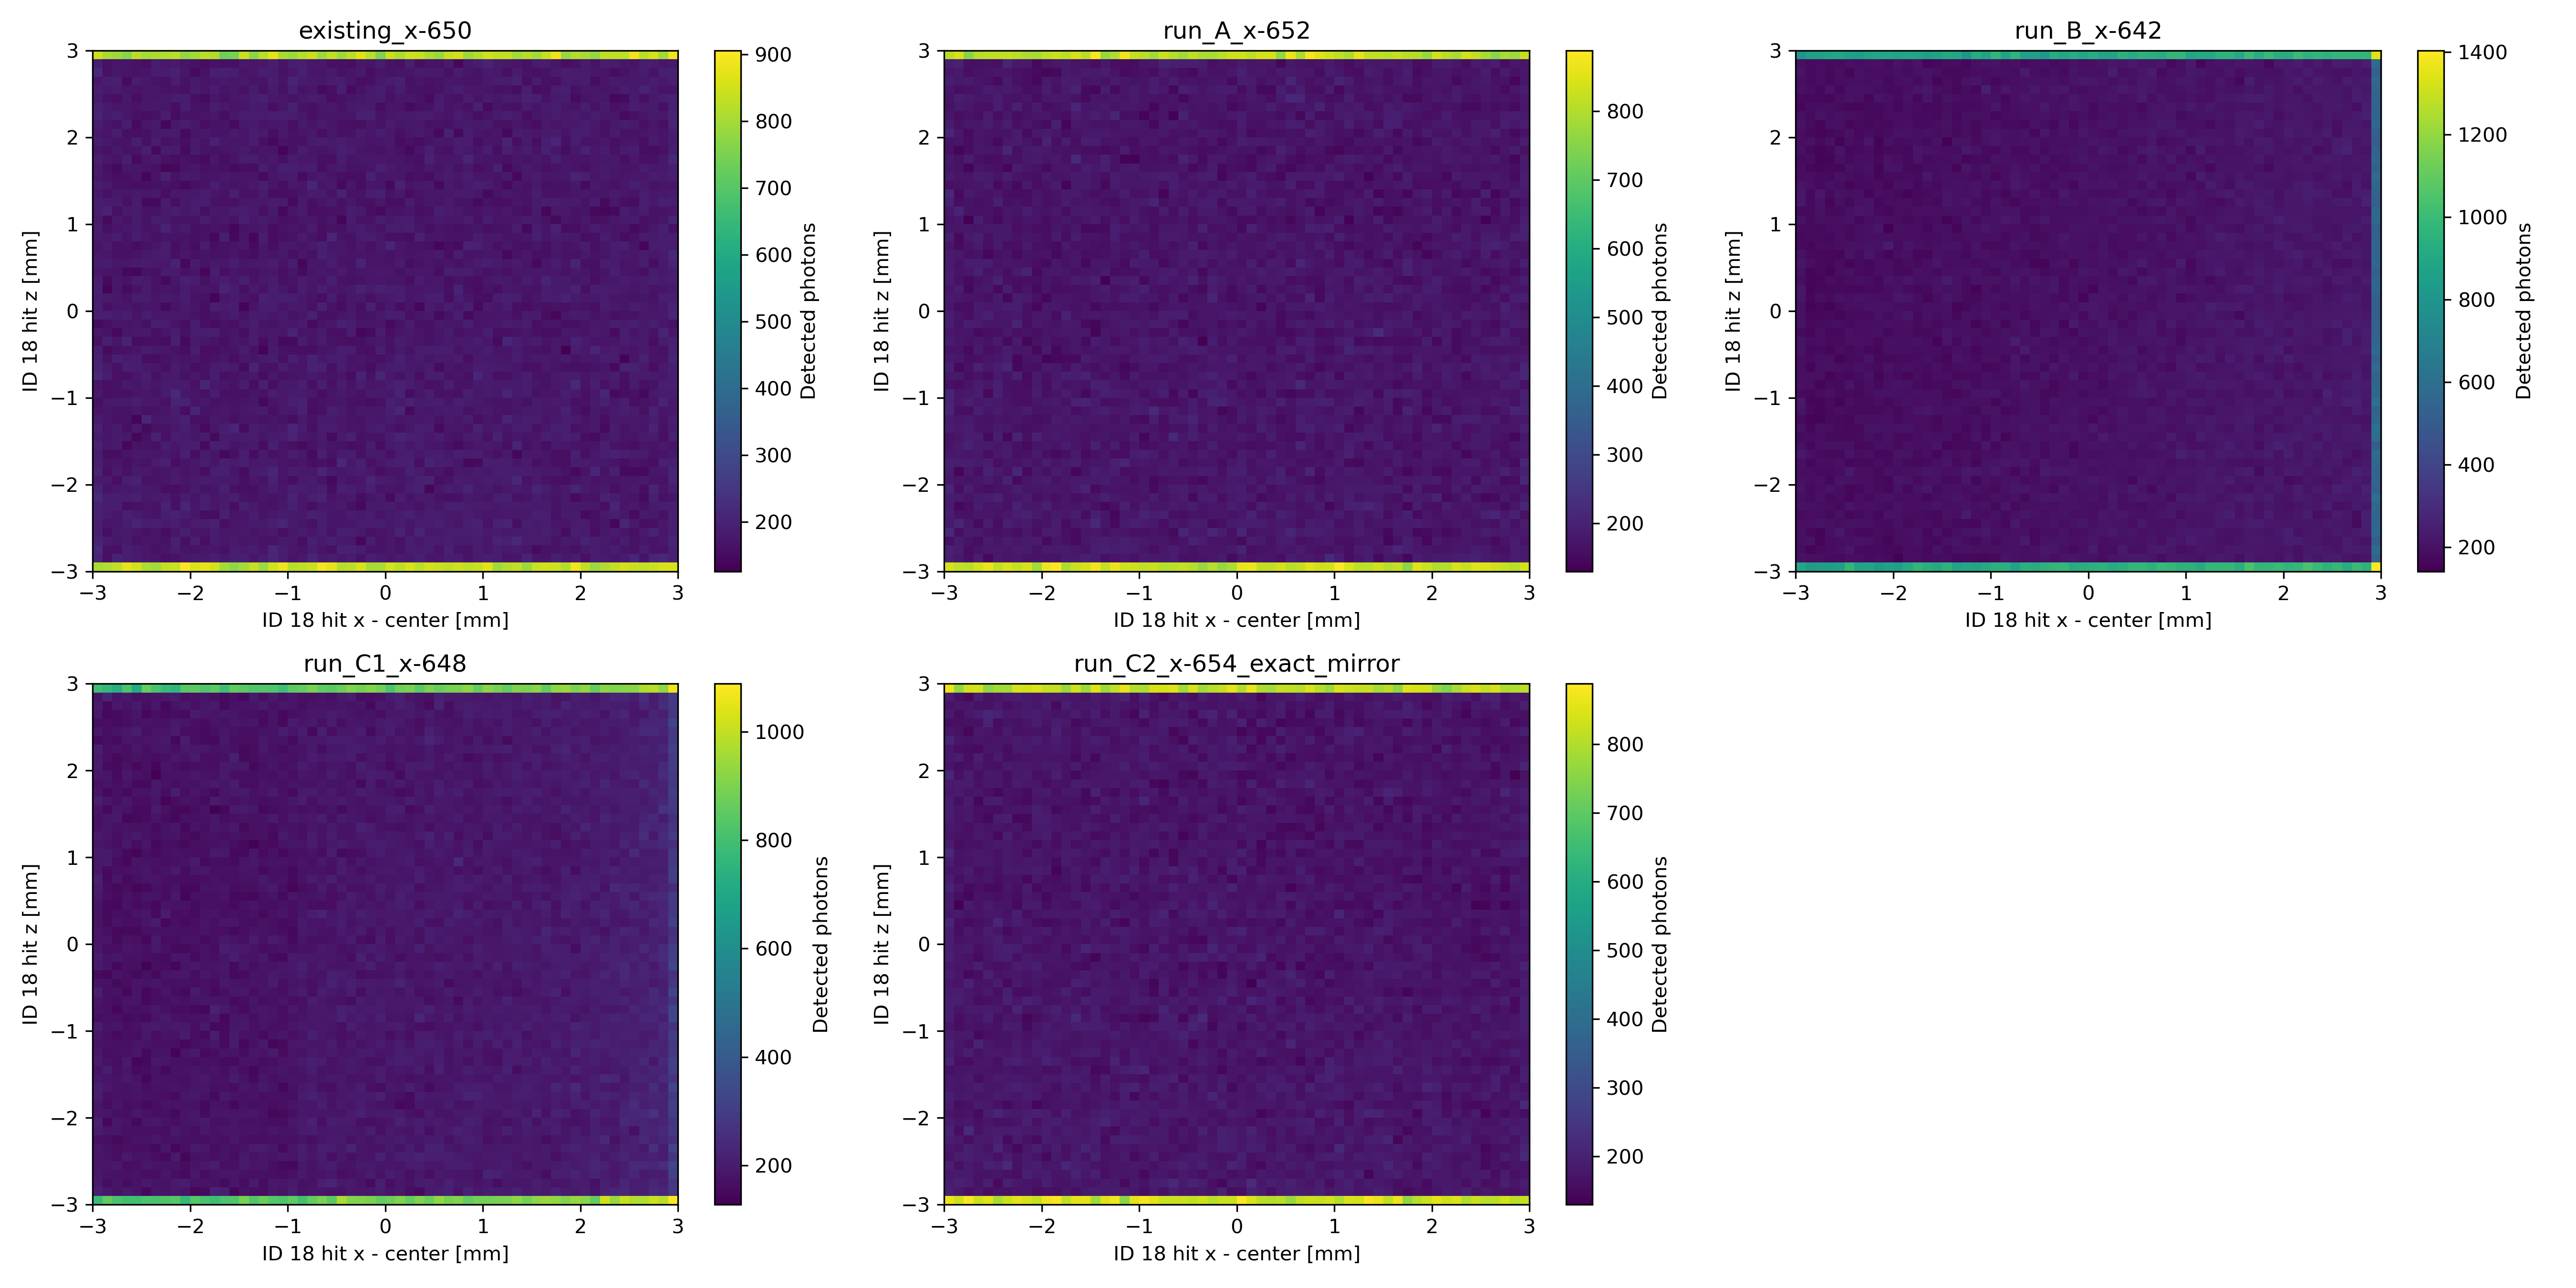
\includegraphics[width=\textwidth,height=0.78\textheight,keepaspectratio]{figs/exec08b_id18_impact_maps.png}
\end{frame}
\begin{frame}{Backup: timing methodology}

\begin{itemize}
 \item SUM4 groups: \{0..3\}, \{4..7\}, \{8..11\}, \{12..15\}.
 \item Single-PE response: normalized 0.5/5 ns double exponential.
 \item Absolute leading-edge threshold: 4 PE equivalent.
 \item Estimator: $\sigma(\Delta T_{AB})/\sqrt{2}$.
 \item \texttt{HOOK\_WALK}: pending; no time-walk correction exists or was invented.
 \item EXEC\_09 anti-artifact audit verifies common threshold, pulse, t=0 and estimator.
\end{itemize}

\end{frame}
\begin{frame}{Backup: EndTop versus End-only tail audit}
\centering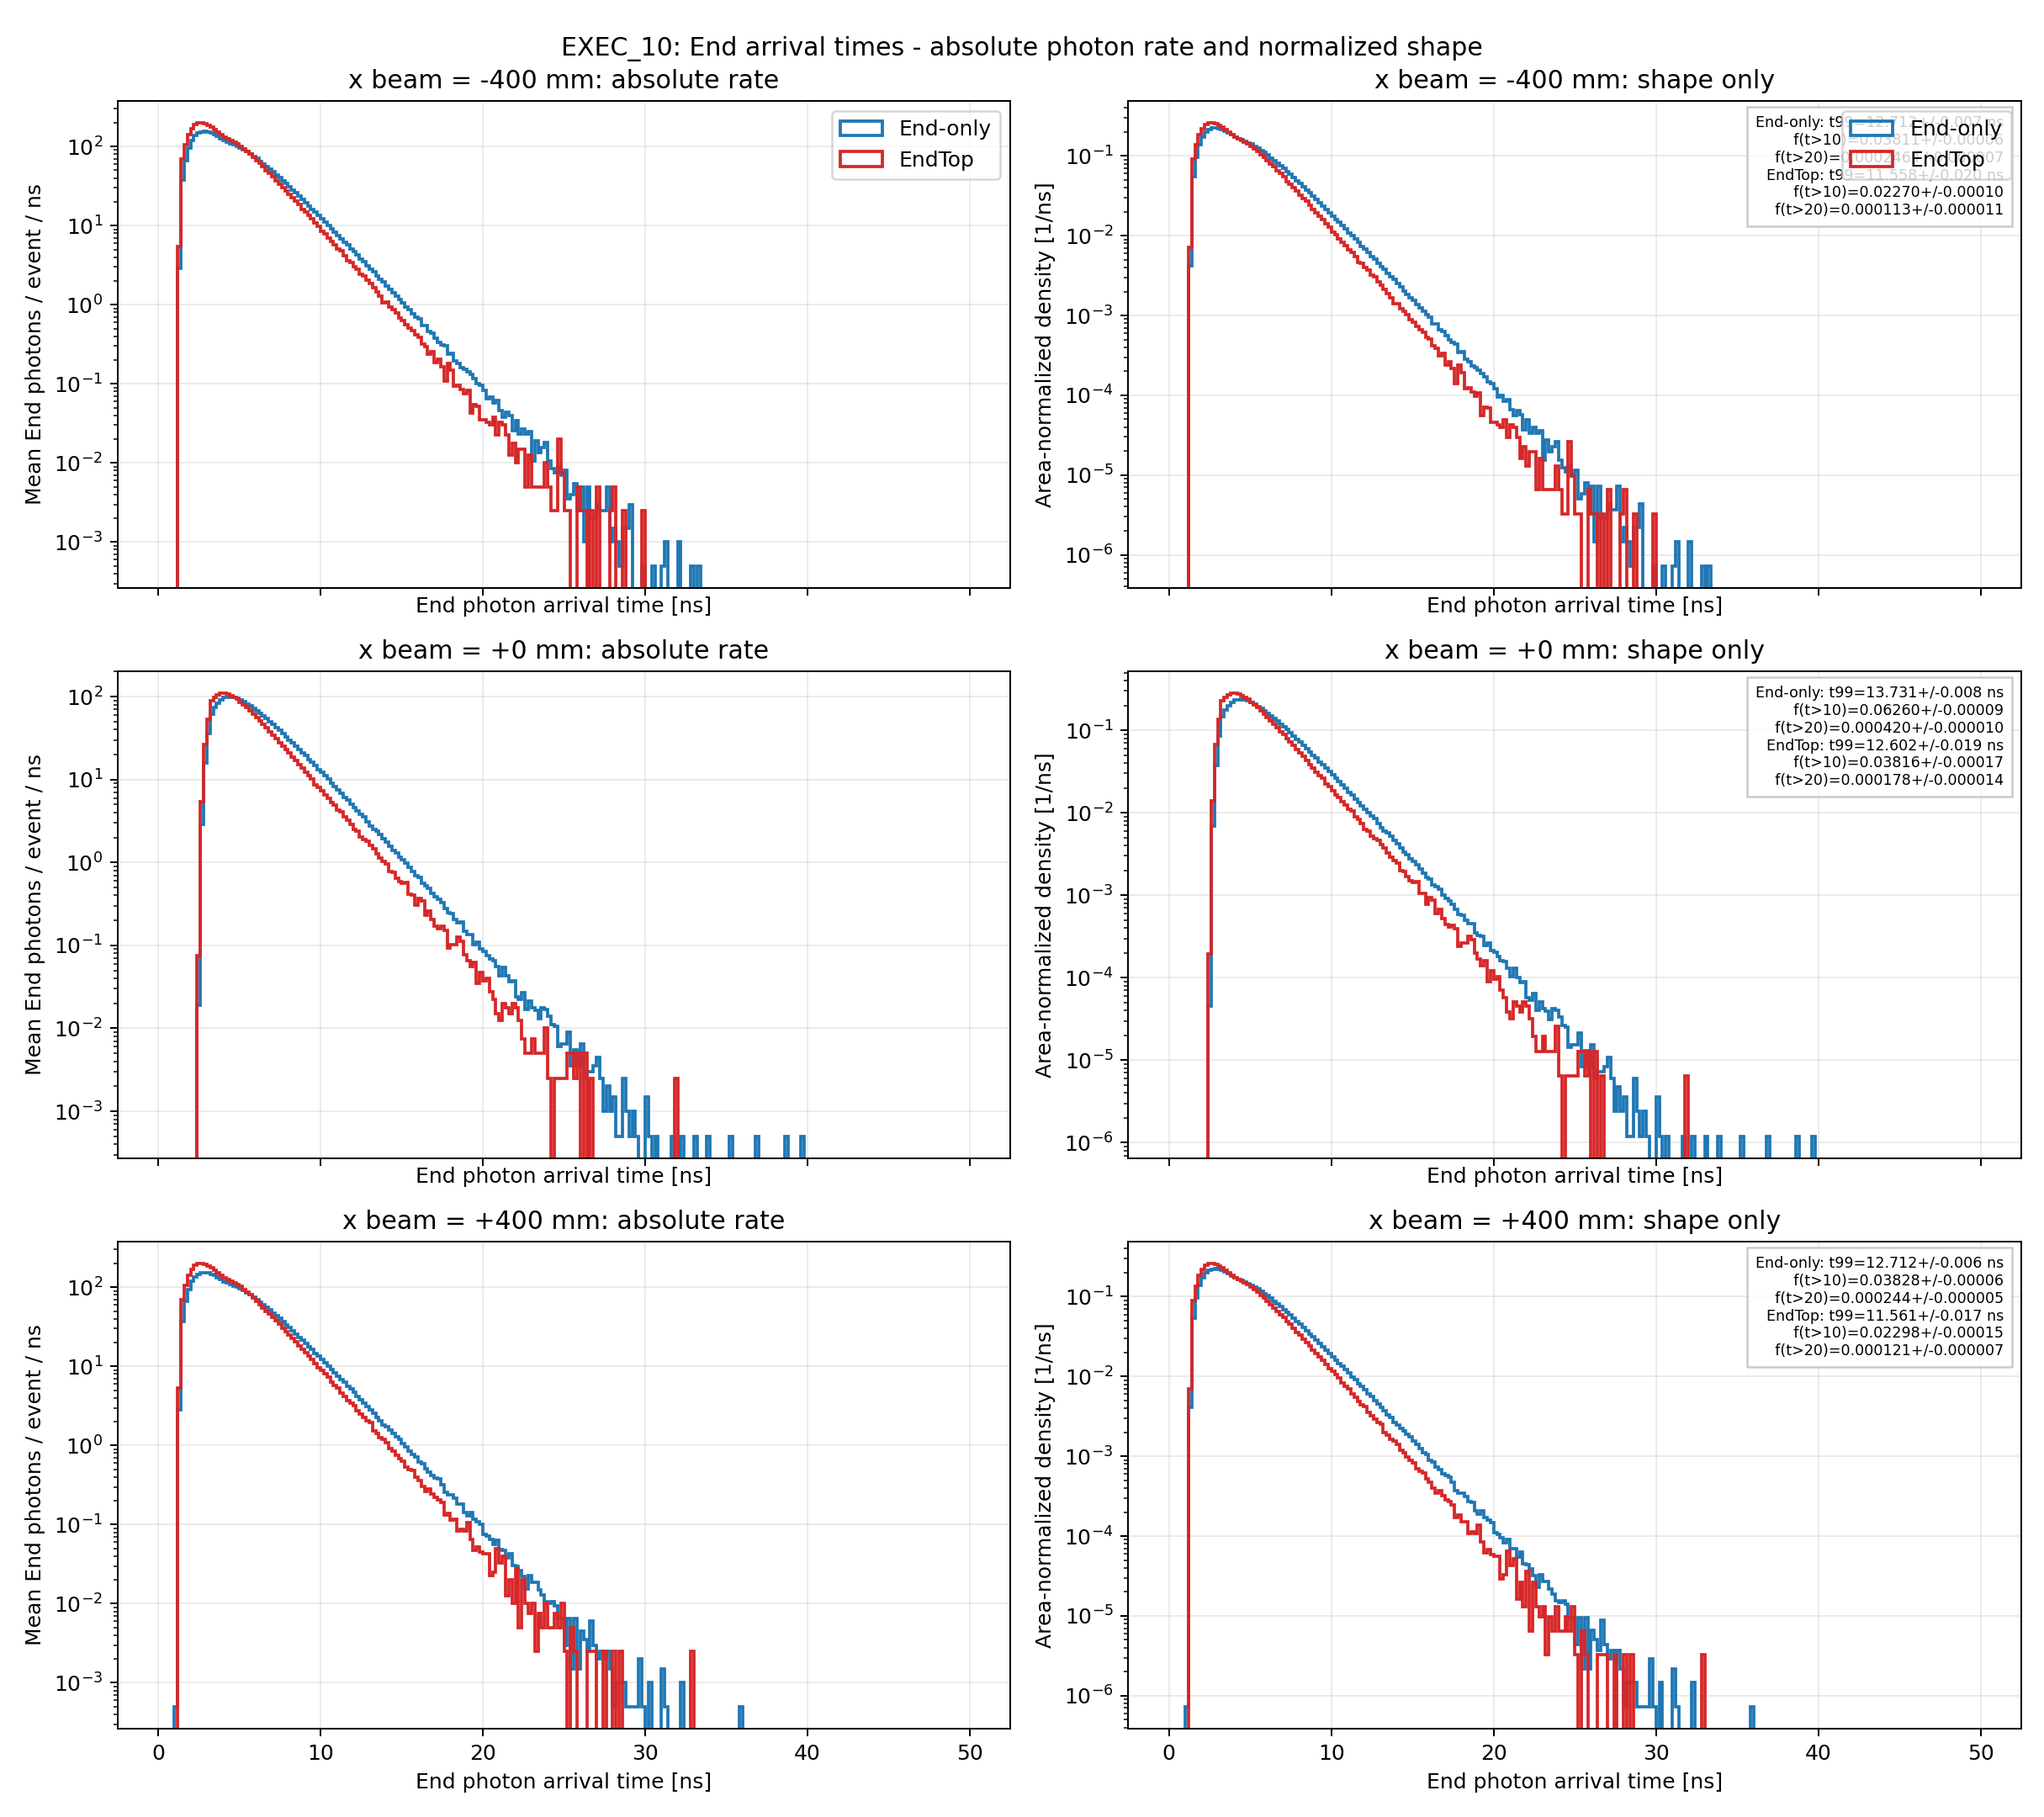
\includegraphics[width=\textwidth,height=0.78\textheight,keepaspectratio]{figs/exec09_tail_comparison.png}
\end{frame}
\end{document}
